\documentclass[conference,compsoc]{IEEEtran}
\AtBeginDocument{%
  \providecommand\BibTeX{{%
    Bib\TeX}}}

\ifCLASSOPTIONcompsoc
  % IEEE Computer Society needs nocompress option
  % requires cite.sty v4.0 or later (November 2003)
  \usepackage[nocompress]{cite}
\else
  % normal IEEE
  \usepackage{cite}
\fi

\ifCLASSINFOpdf
\else
\fi

\newcommand{\ignore}[1]{}

%IEEEtran
\usepackage{amsthm}
\pagestyle{plain}
\usepackage{tcolorbox}
\usepackage{xcolor}
\usepackage{amsmath}

\usepackage{enumitem}
\usepackage{pifont}

\usepackage{subcaption}        
\usepackage{hyperref}

%\usepackage{appendix}
\usepackage{booktabs}    % for \midrule, \toprule, \bottomrule
\usepackage[table]{xcolor} % for \rowcolor
\usepackage{tabularx}

\usepackage[normalem]{ulem}
%\usepackage{url}
\usepackage{xurl}

\usepackage{threeparttable}

\usepackage{listings}

\newtcolorbox{takeawaybox}{
    colback=gray!10,
    colframe=gray!70,
    arc=0pt,
    outer arc=0pt,
    boxrule=0.5pt,
    left=2pt,
    right=2pt,
    top=2pt,
    bottom=2pt,
    before skip=8pt,
    after skip=8pt
}

% correct bad hyphenation here
\hyphenation{op-tical net-works semi-conduc-tor}

\usepackage{graphicx}
\usepackage{makecell}
\usepackage{array}

\newcommand{\para}[1]{\vspace{3pt}\textbf{#1.~}}
\newcommand{\subpara}[1]{\vspace{3pt}\textbf{#1}}

\usepackage{multirow}

\newcommand{\xw}[1] {{\color{red}xueqiang: #1}}
\newcommand{\yao}[1] {{\color{blue}yao: #1}}
\newcommand{\jh}[1] {{\color{violet}jingzhou: #1}}

\definecolor{notepink}{RGB}{0,140,140}
\newcommand{\mycontent}[1] {{\color{notepink}Content: #1}}
\newenvironment{outlinenote}{\par\begingroup\color{red}}{\par\endgroup}

\begin{document}

\title{``I Thought It Was Gone'': Understanding User Data Deletion Experiences, Expectations, and Post-Deletion Data Resurfacing in Commercial LLM Agents}

\maketitle
\begin{abstract}


Commercial LLM agents retain user-provided information across conversations and offer various data deletion methods, yet it remains unclear whether these methods achieve the outcomes users expect.
%
In this study, we investigate users' data deletion practices, expectations, and verification strategies, alongside the post-deletion behavior of commercial LLM agents.
%
We conducted a survey of 177 U.S. adults with prior data deletion experience and developed a Data Injection-Deletion-Recall (DIDR) pipeline to evaluate whether synthetic user information remains retrievable after deletion.
%
Using DIDR, we conducted 865 test cases across six commercial LLM agents, with recall tested at least 30 days after deletion.
%
Our survey reveals that users generally expect deletion methods to permanently remove their information and prevent future retrieval, yet many lack reliable ways to verify deletion outcomes.
%
Our experiments further reveal substantial differences in post-deletion behavior across agents, with information sometimes remaining retrievable despite deletion requests and confirmations.
%
Moreover, post-deletion outcomes varied more across agents than across deletion methods or request wording.
%
By comparing users' expectations with observed agent behavior, we identify discrepancies between expected deletion outcomes and subsequent information retrievability, while finding that agents' responses and interface changes do not reliably indicate recall outcomes.
%
Our findings motivate clearer communication of deletion scope, verifiable deletion feedback, and standardized evaluation protocols to improve data deletion practices in LLM agents.


\end{abstract}


\IEEEpeerreviewmaketitle

\section{Introduction}
\label{sec:intro}

\begin{outlinenote}
\begin{enumerate}[leftmargin=*,nosep]
\item LLM agents remember what users tell them, and that raises the question of deleting it.
\item Privacy law gives a right to deletion, but agents offer many deletion methods with different scopes.
\item Gap: we know little about how users delete, what they expect, or what agents do after a request.
\item Our approach: a participatory survey, plus a pipeline that tests six commercial agents.
\item The four research questions, one line each.
\item Findings in brief, with the user and agent sides placed side by side.
\item Contributions: the survey, the DIDR pipeline, and the comparison of user expectations with agent behavior.
\item Paper roadmap.
\end{enumerate}
\end{outlinenote}



\section{Background}
\label{sec:background}

\para{Legal foundations and user expectations of data deletion}
%
Data deletion is an important mechanism for protecting user privacy, supported by both legal requirements and user expectations. 
%
For example, Article 17 of the GDPR establishes the right to erasure under specified conditions, commonly known as the right to be forgotten~\cite{gdpr2016}. 
%
Similarly, the CCPA gives California residents the right to request deletion of their personal information~\cite{ccpa2018}. 
%
Beyond legal requirements, users expect to have control over their personal information, including the ability to delete previously shared data~\cite{murillo2018if}.
%
As LLM agents accumulate substantial amounts of personal information through ongoing conversations (e.g., voluntary user disclosures and requests for user information to personalize their responses) and may also use user data to train their models, understanding whether and how data deletion works in these systems becomes critical to protecting users' privacy rights.

\para{Data deletion methods of LLM agents}
%
Looking through user-facing features, LLM agents may retain user-provided information across different locations, such as conversation histories, saved memories\footnote{Here, saved memory refers to a user-facing feature that retains information across conversations, rather than information encoded in model parameters or held in the context window.}, and account-level profiles or settings.
%
Accordingly, LLM agents offer different data deletion methods that appear to target specific data storage locations, while their effects on data retained elsewhere are not always clear.
%
For example, deleting a conversation removes it from the user-visible conversation history, but its effects on information retained in saved memories or used for model training remain unclear.


To understand the deletion methods available to users, we conducted a systematic walkthrough of six widely used commercial LLM agents using free consumer accounts:  ChatGPT, Claude, Gemini, Copilot, Perplexity, and DeepSeek.
%
Following prior research on LLM privacy controls~\cite{li2026privacy}, we inspected each agent's interface and settings to identify the available data deletion methods.
%
As shown in Table~\ref{tab:methods}, we identified six data deletion methods: (D1) sending a deletion-request prompt through conversations; (D2) deleting a single conversation or (D3) clearing all conversation history through UI buttons; (D4) deleting a specific saved memory or (D5) clearing all saved memories through memory settings; and (D6) using an account-level privacy dashboard.
%
These methods differ in their intended scope, ranging from individual conversations and saved facts to broader conversation histories and account-level data management.
%
Their availability also varies across agents, as detailed in Table~\ref{tab:methods}.


\begin{table}[t]
\centering
\caption{Availability of six data deletion methods across commercial LLM agents. A dash indicates that a method was unavailable on the tested free account.}
\label{tab:methods}
\footnotesize
\setlength{\tabcolsep}{3pt}
\begin{tabular}{@{}p{0.5\columnwidth}cccccc@{}}
\toprule
Data deletion method
& \rotatebox{75}{ChatGPT}
& \rotatebox{75}{Claude}
& \rotatebox{75}{Gemini}
& \rotatebox{75}{Copilot}
& \rotatebox{75}{Perplexity}
& \rotatebox{75}{DeepSeek} \\
\midrule
(D1) Send a deletion-request prompt
& \ding{51} & \ding{51} & \ding{51} & \ding{51} & \ding{51} & \ding{51} \\
(D2) Delete a single conversation
& \ding{51} & \ding{51} & \ding{51} & \ding{51} & \ding{51} & \ding{51} \\
(D3) Clear all conversation history
& \ding{51} & -- & \ding{51} & -- & \ding{51} & \ding{51} \\
(D4) Delete a specific saved memory
& -- & \ding{51} & \ding{51} & \ding{51} & -- & -- \\
(D5) Clear all saved memories
& \ding{51} & \ding{51} & \ding{51} & \ding{51} & -- & -- \\
(D6) Use a privacy dashboard
& -- & -- & -- & \ding{51} & -- & -- \\
\bottomrule
\end{tabular}
\end{table}
\section{Understanding User Data Deletion Practices and Expectations}
\label{sec:user_study}

To investigate users' data deletion practices and expectations in LLM agents (RQ1 and RQ2), we conducted an online survey of users with prior experience deleting data from LLM agents.
%
This section describes our study methodology and presents the key findings.

\subsection{User Study Methodology}

\subsubsection{Participant Recruitment}
%
We recruited participants through Prolific, targeting adults aged 18 or older residing in the United States who had used at least one of the six LLM agents described in Section~\ref{sec:background}. 
%
The survey was administered through Qualtrics, with a recruitment target of approximately 200 participants to support the exploratory nature of the study.
%
Participants received \$4 upon completing the survey and passing the attention checks.
%
Of 235 submissions, we excluded 36 participants who reported no prior experience deleting data from LLM agents, as our analysis focused on users with such experience. 
%
We further excluded 17 incomplete submissions, one response that failed an attention check, and four participants with missing responses to key survey questions, yielding a final sample of 177 participants.
%
Among these participants, 58.8\% were men, 40.7\% were women (one preferred not to say), 73.4\% were under 45 years old, and 62.1\% held at least a bachelor's degree (Table~\ref{tab:demographics}). 
%
Thus, our survey findings characterize users with prior deletion experience rather than the broader population of LLM-agent users.
%
Separately, we collected deletion-request prompts from 209 participants, including some without prior deletion experience, for the later post-deletion analysis in Section~\ref{sec:didr}, as the hypothetical prompt-writing task did not require such experience.
%
Table~\ref{tab:demographics} in the Appendix presents the demographic details of the participants.

\subsubsection{Study Procedure}
%
The survey was designed to take about 15 minutes to complete. 
%
Participants first reviewed an informed consent form describing the study's purpose, procedures, data handling, and participant rights. 
%
Those who consented proceeded to screening questions assessing their age, U.S. residence, and prior use of LLM agents.
%
Eligible participants then completed the following survey components in sequence: (1) LLM-agent usage and prior use of deletion methods; (2) scenario-based assessments of deletion practices, expectations, and verification; (3) prior data deletion experiences; (4) deletion feedback and desired confirmation mechanisms; (5) privacy awareness and knowledge; (6) attitudes toward LLM agents, data sharing, social influences, and perceived AI-related abilities; and (7) demographic information.
%
The scenario-based assessments involved two scenarios presented in randomized order, each followed by the same set of questions. 
%
Two instructed-response attention checks were embedded in the survey to assess response quality. Throughout the survey, we used the term ``AI chatbot'' to refer to LLM agents, as this term is more familiar and accessible to general users.

\subsubsection{Survey Question Design}
%
\label{subsubsec:questions}
%
We designed the survey questions to investigate users' deletion practices (RQ1) and their expectations and verification strategies (RQ2), using scenario-based assessments complemented by questions about prior experiences.

\para{Scenario design}
%
To investigate users' deletion practices and how these practices vary across different contexts, we developed two hypothetical scenarios involving different levels of data sensitivity and usage contexts.
%
The less sensitive scenario (\textbf{LS}) concerns sharing a city while requesting weather information, whereas the more sensitive scenario (\textbf{MS}) concerns disclosing a home address while seeking a clinic for sexually transmitted infection treatment.
%
In both scenarios, participants were asked to consider deleting the disclosed location information to protect their privacy. 
%
The scenarios used identical follow-up questions and were presented in randomized order to enable within-participant comparisons while mitigating potential order effects.

\para{Data deletion practices (RQ1)}
%
Before evaluating the scenarios, participants were introduced to eight deletion methods, including the six methods described in Table~\ref{tab:methods}, account deletion, and filing a deletion request.
%
Each method was accompanied by a description and example screenshot. 
%
Participants reported which methods they had previously used.
%
For each scenario, participants selected a deletion method from those they had previously used and explained their choice. 
%
They then rated the selected method along three dimensions using five-point agreement scales: \textit{perceived privacy protection} (five items), \textit{effort} (four items), and \textit{potential loss of personalized benefits} (three items). 
%
Participants also indicated their willingness to delete the disclosed information on a five-point scale. 
%
Finally, they selected their preferred deletion methods from all available options, regardless of prior experience, allowing us to distinguish prior method use from hypothetical preferences.

\para{User expectations and verification (RQ2)}
%
For each scenario, participants indicated what they expected their selected deletion method to accomplish, including \textit{permanent deletion from the database and backups}, being \textit{made invisible to users}, the agent not referencing the information in \textit{the current conversation} or in \textit{future conversations}, and \textit{exclusion from model training}. 
%
Participants could select multiple outcomes or indicate uncertainty.
%
We also asked participants how they had previously verified deletion, including asking the agent in the same or a new conversation, checking saved memories or the user interface, and submitting a data access request through a privacy portal. 
%
Participants could indicate that they did not know how to verify deletion or did not wish to do so, and rated their confidence in verification. 
%
Additional questions examined the confirmation participants had received after previous deletion attempts and the feedback they believed LLM agents should provide.

\para{Participant-authored deletion-request prompts}
%
In each scenario, participants wrote the message they would send to an LLM agent to request deletion of the disclosed information and explained their wording. 
%
These participant-authored deletion-request prompts were later used as inputs to our post-deletion analysis (RQ3; Section~\ref{sec:didr}), allowing us to evaluate LLM agents using prompts written by survey participants (i.e., real users).

\para{Other survey questions}
%
We also asked participants about their prior deletion experiences, including the types of information they had attempted to delete, their motivations, how they discovered deletion controls, and whether agents had subsequently referenced information they believed was deleted.
%
Finally, we collected participants' demographic characteristics, including education level, gender, and primary domain of work or study. 
%
To assess response quality, we also embedded two instructed-response attention checks in the survey, asking participants to select a specific response option to verify that they were reading and following the instructions carefully.
%
The complete questionnaire, including question wording and measurement items, is provided in Appendix~\ref{app:questions}.


\subsubsection{Data Analysis}
%
We analyzed responses from 177 participants, reporting percentages separately for the less sensitive (LS) and more sensitive (MS) scenarios. 
%
Because each participant evaluated both scenarios, we used paired statistical tests to compare their responses. 
%
Specifically, we used Wilcoxon signed-rank tests~\cite{wilcoxon1945individual} for \textit{willingness to delete}, \textit{perceived privacy protection}, \textit{effort}, and \textit{benefit loss}; the Stuart-Maxwell test~\cite{agresti2013categorical} for overall deletion-method choices; and McNemar tests~\cite{agresti2013categorical} for individual deletion methods, expected deletion outcomes, and verification strategies. 
%
We also examined potential scenario-order effects using binomial~\cite{agresti2013categorical}, Mann-Whitney~\cite{mann1947test}, and Fisher's exact tests~\cite{agresti2013categorical}. 
%
To compare deletion methods, we pooled responses from both scenarios (\textbf{Pooled}), with each participant contributing two responses. 
%
We fitted generalized estimating equations (GEE)~\cite{liang1986longitudinal} clustered by participant to account for within-participant dependence. 
%
To avoid unstable estimates from small groups, we restricted these analyses to the four deletion methods selected by at least 14 participants, retaining 317 of the 354 responses. 
%
We used Gaussian models~\cite{liang1986longitudinal} for \textit{perceived privacy protection}, \textit{effort}, and \textit{benefit loss}, and logistic models~\cite{agresti2013categorical} for binary expectation outcomes, with scenario included as a covariate. 
%
Pairwise differences in effort were assessed using GEE contrasts, while verification strategies were compared across methods using chi-square or Fisher's exact tests separately for each scenario.


We assessed the three perception scales using confirmatory factor analysis (CFA), with separate factors for protection (five items), effort (four items), and benefit loss (three items).
%
Standardized factor loadings ranged from .73 to .94, average variance extracted from .64 to .76, and Cronbach's $\alpha$ from .87 to .92. Model fit was acceptable on several indices (CFI = .94, TLI = .92, SRMR = .060), although RMSEA = .099 exceeded the conventional .08 threshold. 
%
Because the pooled CFA did not account for repeated responses, we also fitted separate models for each scenario, obtaining similar results (CFI = .95 and .93; RMSEA = .087 and .108). 
%
We treated the analyses as exploratory and applied Holm corrections~\cite{holm1979simple} within families of related tests, leaving individual tests unadjusted. 
%
We report adjusted values as $p_{\mathrm{Holm}}$. 
%
Table~\ref{tab:analysis-families} summarizes the statistical tests, sample sizes, and correction families.

\begin{table*}[t]
\centering
\caption{Summary of statistical analyses, tests, and multiple-testing correction families.}
\label{tab:analysis-families}
\small
\begin{tabular}{@{}p{0.32\textwidth}p{0.28\textwidth}p{0.20\textwidth}p{0.14\textwidth}@{}}
\toprule
Analysis & Statistical test & Sample & Holm family \\
\midrule

\multicolumn{4}{@{}l}{\textit{Scenario comparisons (LS vs. MS)}} \\
Willingness to delete
    & Wilcoxon signed-rank; rank-biserial $r$
    & 177 pairs
    & None (single test) \\
Protection, effort, and benefit loss
    & Wilcoxon signed-rank; rank-biserial $r$
    & 177 pairs
    & 3 scales \\
Deletion-method choice (overall)
    & Stuart-Maxwell marginal homogeneity
    & 176 participants who chose a method in both scenarios
    & None (single test) \\
Deletion-method choice (each method)
    & McNemar
    & 177 participants
    & 7 methods \\
Expected deletion outcomes
    & McNemar
    & 177 participants
    & 7 options \\
Verification strategies
    & McNemar
    & 177 participants
    & 8 options \\
\midrule

\multicolumn{4}{@{}l}{\textit{Deletion-method comparisons}} \\
Protection, effort, and benefit loss
    & Gaussian GEE, clustered by participant (Wald)
    & 317 responses, 4 methods
    & 3 scales \\
Effort (pairwise between methods)
    & GEE contrasts, adjusted for scenario
    & 317 responses, 4 methods
    & 6 method pairs \\
Expected deletion outcomes
    & Logistic GEE, clustered by participant
    & 317 responses, 4 methods
    & 7 options \\
Verification strategies
    & Chi-square or Fisher's exact, each scenario separately
    & Participants choosing a method with at least 14 participants in that scenario
    & 8 options, within each scenario \\
\midrule

\multicolumn{4}{@{}l}{\textit{Measurement validation and robustness checks}} \\
Scale structure
    & Confirmatory factor analysis
    & 354 responses
    & Not applicable \\
Scenario order
    & Binomial test, Mann-Whitney, Fisher's exact
    & 177 participants
    & 4 ratings (Mann-Whitney) \\
\bottomrule
\end{tabular}

\par\vspace{0.5em}
\begin{minipage}{0.94\textwidth}
\footnotesize
\textit{Note.} LS and MS denote the less and more sensitive scenarios, respectively.
A response is one participant's answer in one scenario.
GEE denotes generalized estimating equations.
Holm corrections are applied within the specified families;
single tests are not adjusted.
\end{minipage}
\end{table*}

\subsection{User Study Findings}
\label{sec:qual_results}

We present findings from 177 participants, organized around users' deletion practices (RQ1) and their expectations and verification strategies (RQ2).
%
Results are reported separately for the less sensitive (LS) and more sensitive (MS) scenarios.
%
Analyses combining both scenarios are denoted as \textbf{Pooled}, comprising 354 responses unless otherwise specified.

\subsubsection{User Deletion Practices (RQ1)}

Deleting a single conversation was the most commonly used deletion method (76.8\% of participants) and the most frequently selected method in both scenarios (Table~\ref{tab:method-use}).
%
Clearing all conversation history was also common (53.1\%), whereas deleting a specific saved memory (32.2\%) and clearing all saved memories (25.4\%) were less frequently reported.
%
Fewer participants had used a privacy dashboard (9.6\%), deleted their account (10.2\%), or filed a deletion request (2.8\%).
%
Most participants discovered deletion controls by exploring the settings or guessing how to delete their data, while only 6 of 177 reported learning about these options from the agent itself.

\begin{table*}[!t]
\centering
\caption{Previously used deletion methods (multiple selections allowed) and scenario-based method choices in LS, MS, and Pooled. Scenario-based choices were restricted to methods participants had previously used; ``Other'' choices are excluded from the pooled counts.}
\label{tab:method-use}
\small
\begin{tabular}{@{}lrrrr@{}}
\toprule
 & Previously used & \multicolumn{3}{c}{Chosen in scenario} \\
\cmidrule(lr){3-5}
Deletion method & ($n=177$) & LS & MS & Pooled ($n=352$) \\
\midrule
Sending a deletion-request prompt & 55 (31.1\%) & 25 & 14 & 39 (11.1\%) \\
Deleting a single conversation & 136 (76.8\%) & 84 & 80 & 164 (46.6\%) \\
Clearing all conversation history & 94 (53.1\%) & 33 & 40 & 73 (20.7\%) \\
Deleting a specific saved memory & 57 (32.2\%) & 19 & 22 & 41 (11.6\%) \\
Clearing all saved memories & 45 (25.4\%) & 7 & 8 & 15 (4.3\%) \\
Using a privacy dashboard & 17 (9.6\%) & 6 & 9 & 15 (4.3\%) \\
Deleting the account & 18 (10.2\%) & 2 & 3 & 5 (1.4\%) \\
Filing a request & 5 (2.8\%) & 0 & 0 & 0 (0.0\%) \\
\bottomrule
\end{tabular}
\end{table*}

The more sensitive scenario increased participants' willingness to delete the disclosed information, but did not significantly change their deletion-method choices.
%
In LS and MS, respectively, 125 and 150 of 177 participants indicated that they would probably or definitely delete the information.
%
Mean willingness increased from 3.98 in LS to 4.37 in MS on the five-point scale (Wilcoxon signed-rank test, $p<.001$, $r=.55$).
%
However, the overall distribution of deletion-method choices did not differ significantly between scenarios (Stuart-Maxwell test, $p=.39$, 176 participants).
%
Thus, although participants expressed greater willingness to delete information in the more sensitive scenario, we found no corresponding evidence of a change in their selected deletion methods.

Participants' preferred deletion methods also differed from their scenario-based choices.
%
Sending a deletion-request prompt was the second most frequently preferred method (47\%--50\% across LS and MS), following deleting a single conversation (61\%--66\%).
%
However, only 8\%--14\% of participants selected a deletion-request prompt from the methods they had previously used.
%
This gap suggests that deletion-request prompts appealed to many participants, even though relatively few had previously used them.

\begin{takeawaybox}
\textbf{Finding 1:} Participants primarily used conversation-level deletion methods and often discovered deletion controls on their own. The more sensitive scenario increased willingness to delete but did not significantly change deletion-method choices. Although many participants preferred deletion-request prompts, relatively few selected them among their previously used methods.
\end{takeawaybox}


\subsubsection{User Expectations and Verification (RQ2)}

Participants expressed similar expectations across deletion methods, despite differences in the data locations these methods target.
%
Across Pooled responses, 59.0\% expected permanent deletion from the agent's databases and backups, while 54.2\% expected the information to become unavailable for recall in future conversations (Figure~\ref{fig:expectation}).
%
Among the four most frequently selected methods, we detected no statistically significant differences in expectations of permanent deletion ($p_{\mathrm{Holm}}=1.0$) or prevention of recall in future conversations ($p_{\mathrm{Holm}}=1.0$).
%
These results suggest that participants did not consistently distinguish deletion methods by their expected outcomes.
%
In contrast, participants perceived differences in the effort required by deletion methods.
%
Among the four most frequently selected methods, perceived effort differed significantly ($p_{\mathrm{Holm}}=.0001$), whereas perceived privacy protection did not ($p_{\mathrm{Holm}}=.29$; Figure~\ref{fig:scales}).
%
These results suggest that participants differentiated methods more by perceived effort than by expected protection.
%
However, because participants selected their own methods and the groups were relatively small, these comparisons are associative rather than causal.

\begin{figure}[t]
    \centering
    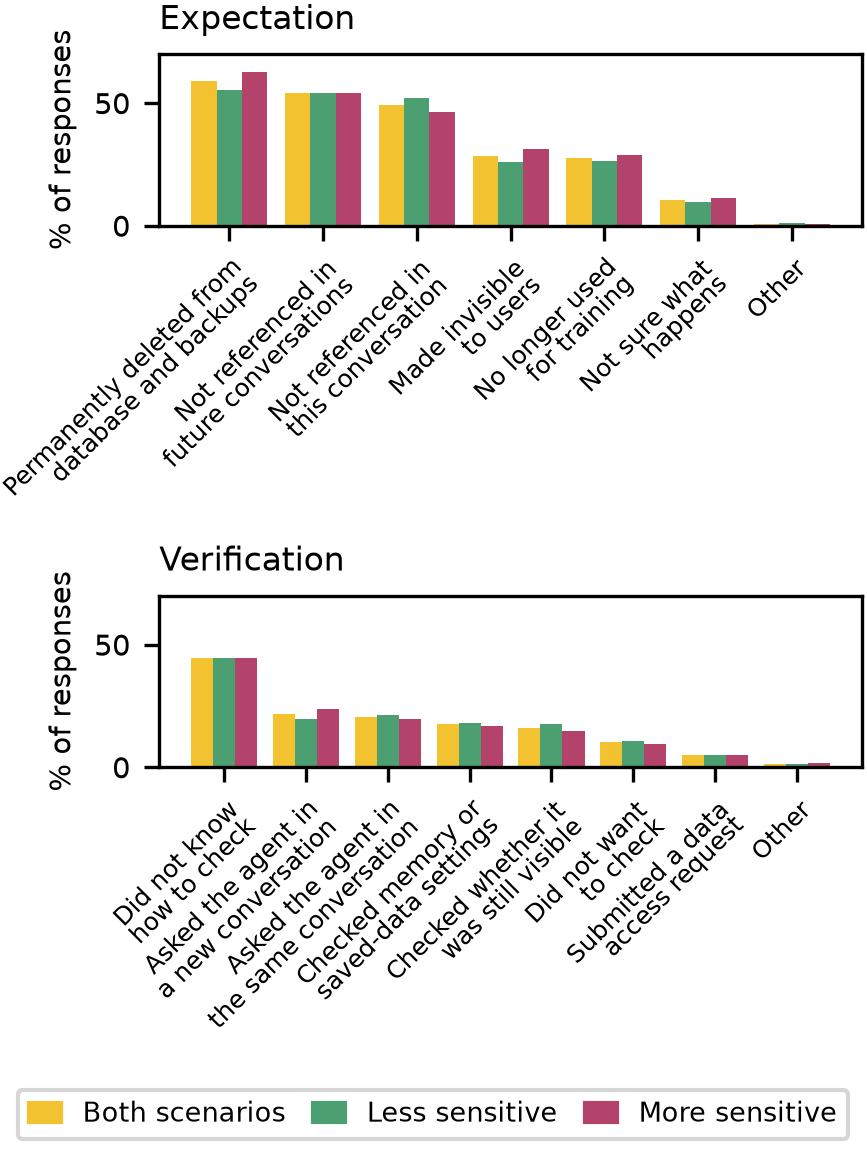
\includegraphics[width=\columnwidth,height=0.42\textheight,keepaspectratio]{figures/fig_expectation.png}
    \caption{Expected deletion outcomes and reported verification strategies in LS, MS, and Pooled. The analysis includes 354 responses from 177 participants, with multiple selections allowed. Percentages are based on 177 participants within each scenario and 354 responses for Pooled results.}
    \label{fig:expectation}
\end{figure}


\begin{figure*}[t]
    \centering
    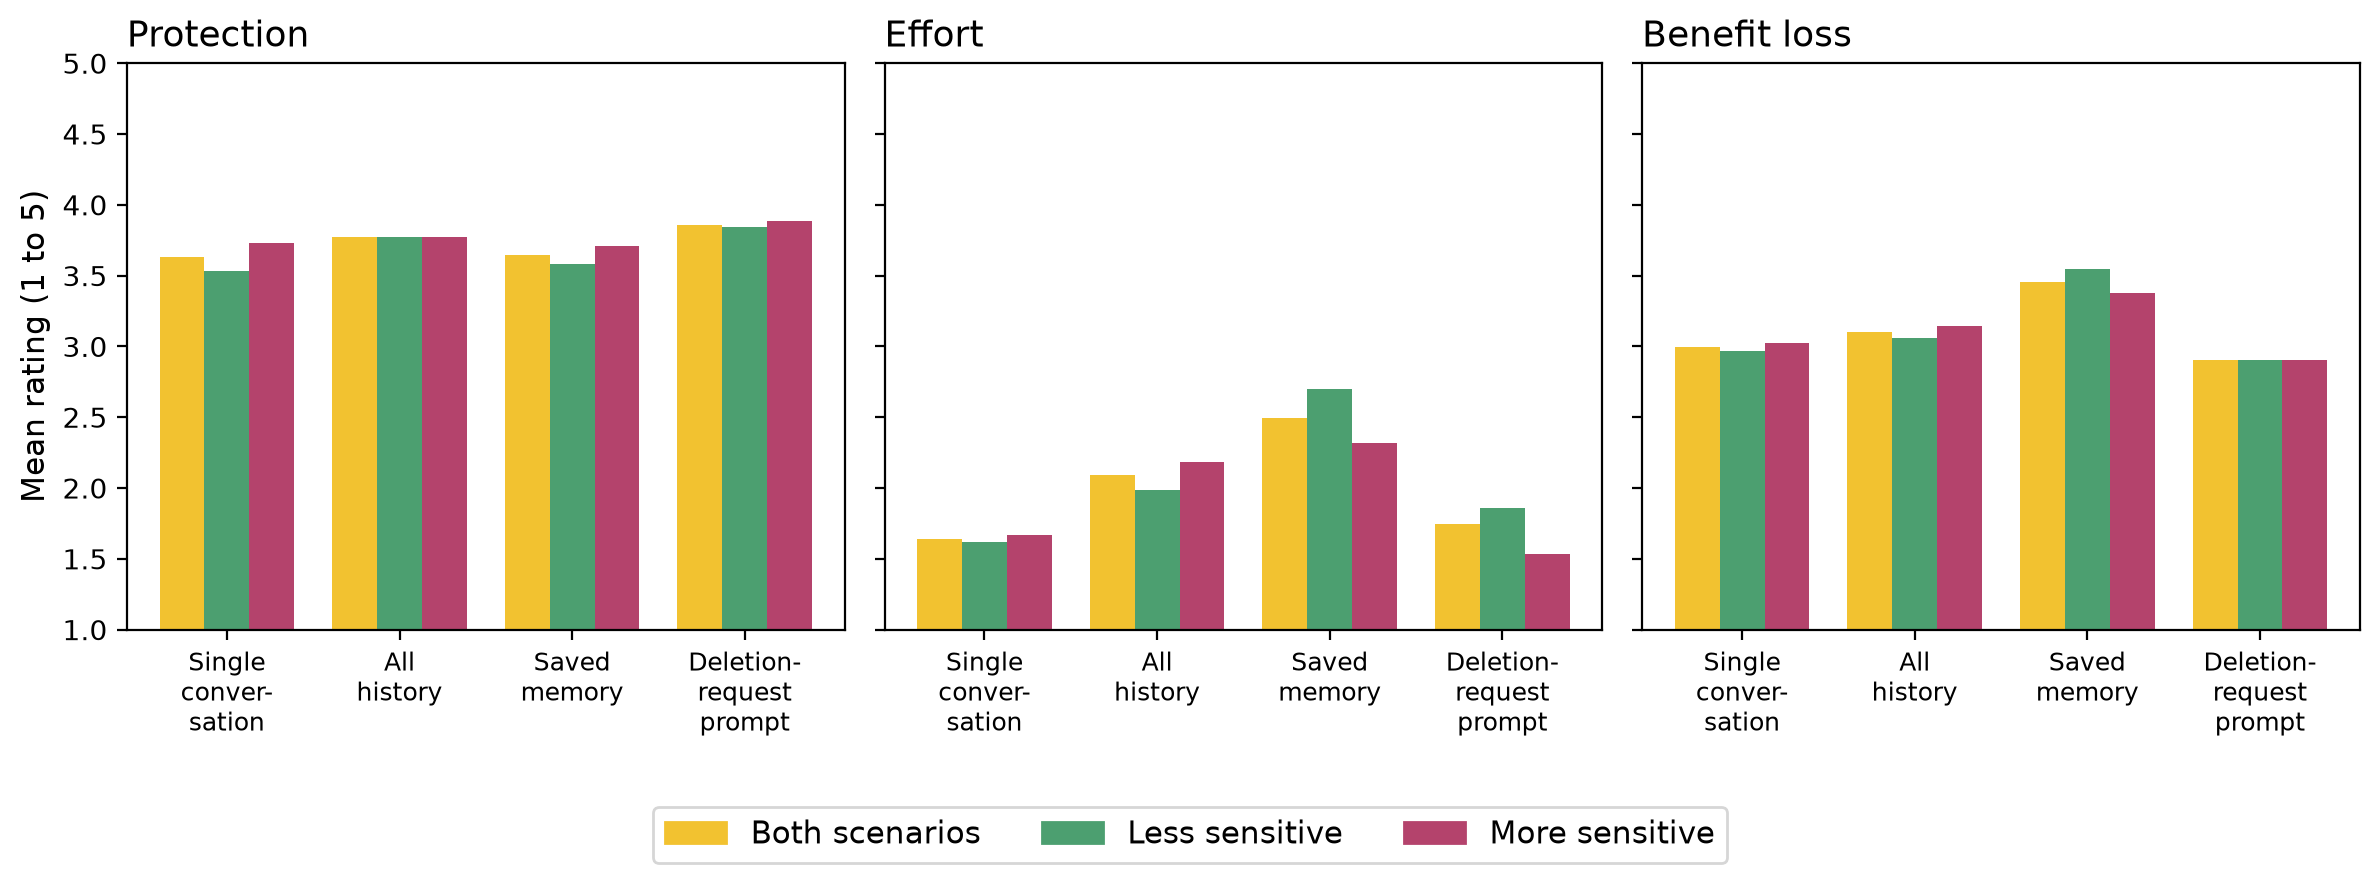
\includegraphics[width=0.9\textwidth]{figures/fig_scales.png}
    \caption{Mean ratings of perceived privacy protection, effort, and potential loss of personalized benefits for the four most frequently selected deletion methods, shown separately for LS and MS and combined (Pooled). The analysis includes 317 responses from 105, 50, 30, and 29 participants, respectively. Ratings use five-point agreement scales.}
    \label{fig:scales}
\end{figure*}

Many participants were uncertain how to verify deletion outcomes.
%
Across Pooled responses, 44.6\% indicated that they did not know how to verify deletion.
%
Reported verification strategies included asking the agent in the same or a new conversation (21\%--22\% of responses) and checking saved memories, settings, or the user interface (16\%--18\%).
%
Notably, among responses selecting a deletion-request prompt, 53.8\% (of 39 responses) indicated verification by asking the agent in the same conversation.
%
This suggests that users relying on conversational deletion requests may also rely on the agent's own responses as evidence that deletion succeeded.

Participants also reported limitations in deletion feedback and experiences of information resurfacing.
%
Among the 177 participants, 42 (23.7\%) reported that an agent had referenced information they believed was deleted.
%
After previous deletion attempts, 41.2\% reported receiving a clear confirmation message, while 29.4\%--34.5\% reported vague acknowledgements or no feedback (multiple selections allowed).
%
Furthermore, 73 participants (41.2\%) wanted a breakdown specifying what information had been deleted and what might still be retained.
%
These findings highlight a gap between users' expectations of deletion and their ability to establish its outcome, motivating our subsequent post-deletion analysis (Section~\ref{sec:tech_analysis}).

%
\begin{takeawaybox}
\textbf{Finding 2:} Participants commonly expected deletion methods to permanently remove their data, despite differences in the data locations these methods target. Perceived effort differed across methods, but expected deletion outcomes and perceived protection showed no significant differences. Many participants did not know how to verify deletion, and those selecting deletion-request prompts often relied on the agent itself for verification.
\end{takeawaybox}












% \section{Understanding User Data Deletion Practices and Expectations}
% \label{sec:user_study}

% To investigate users' data deletion practices and expectations in LLM agents (RQ1 and RQ2), we conducted an online survey of users with prior experience deleting data from LLM agents.
% %
% This section describes our study methodology and presents the key findings.

% \subsection{User Study Methodology}

% \subsubsection{Participant Recruitment}
% %
% We recruited participants through Prolific, targeting adults aged 18 or older residing in the United States who had used at least one of the six LLM agents described in Section~\ref{sec:background}. 
% %
% The survey was administered through Qualtrics, with a recruitment target of approximately 200 participants to support the exploratory nature of the study.
% %
% Participants received \$4 upon completing the survey and passing the attention checks.
% %
% Of 235 submissions, we excluded 36 participants who reported no prior experience deleting data from LLM agents, as our analysis focused on users with such experience. 
% %
% We further excluded 17 incomplete submissions, one response that failed an attention check, and four participants with missing responses to key survey questions, yielding a final sample of 177 participants.
% %
% Among these participants, 58.8\% were men, 40.7\% were women (one preferred not to say), 73.4\% were under 45 years old, and 62.1\% held at least a bachelor's degree (Table~\ref{tab:demographics}). 
% %
% Thus, our survey findings characterize users with prior deletion experience rather than the broader population of LLM-agent users.
% %
% Separately, we collected deletion-request prompts from 209 participants, including some without prior deletion experience, for the later post-deletion analysis in Section~\ref{sec:didr}, as the hypothetical prompt-writing task did not require such experience.
% %
% Table~\ref{tab:demographics} in the Appendix presents the demographic details of the participants.

% \subsubsection{Study Procedure}
% %
% The survey was designed to take about 15 minutes to complete. 
% %
% Participants first reviewed an informed consent form describing the study's purpose, procedures, data handling, and participant rights. 
% %
% Those who consented proceeded to screening questions assessing their age, U.S. residence, and prior use of LLM agents.
% %
% Eligible participants then completed the following survey components in sequence: (1) LLM-agent usage and prior use of deletion methods; (2) scenario-based assessments of deletion practices, expectations, and verification; (3) prior data deletion experiences; (4) deletion feedback and desired confirmation mechanisms; (5) privacy awareness and knowledge; (6) attitudes toward LLM agents, data sharing, social influences, and perceived AI-related abilities; and (7) demographic information.
% %
% The scenario-based assessments involved two scenarios presented in randomized order, each followed by the same set of questions. 
% %
% Two instructed-response attention checks were embedded in the survey to assess response quality. Throughout the survey, we used the term ``AI chatbot'' to refer to LLM agents, as this term is more familiar and accessible to general users.

% \subsubsection{Survey Question Design}
% %
% \label{subsubsec:questions}
% %
% We designed the survey questions to investigate users' deletion practices (RQ1) and their expectations and verification strategies (RQ2), using scenario-based assessments complemented by questions about prior experiences.

% \para{Scenario design}
% %
% To investigate users' deletion practices and how these practices vary across different contexts, we developed two hypothetical scenarios involving different levels of data sensitivity and usage contexts.
% %
% The less sensitive scenario (\textbf{LS}) concerns sharing a city while requesting weather information, whereas the more sensitive scenario (\textbf{MS}) concerns disclosing a home address while seeking a clinic for sexually transmitted infection treatment.
% %
% In both scenarios, participants were asked to consider deleting the disclosed location information to protect their privacy. 
% %
% The scenarios used identical follow-up questions and were presented in randomized order to enable within-participant comparisons while mitigating potential order effects.

% \para{Data deletion practices (RQ1)}
% %
% Before evaluating the scenarios, participants were introduced to eight deletion methods, including the six methods described in Table~\ref{tab:methods}, account deletion, and filing a deletion request.
% %
% Each method was accompanied by a description and example screenshot. 
% %
% Participants reported which methods they had previously used.
% %
% For each scenario, participants selected a deletion method from those they had previously used and explained their choice. 
% %
% They then rated the selected method along three dimensions using five-point agreement scales: \textit{perceived privacy protection} (five items), \textit{effort} (four items), and \textit{potential loss of personalized benefits} (three items). 
% %
% Participants also indicated their willingness to delete the disclosed information on a five-point scale. 
% %
% Finally, they selected their preferred deletion methods from all available options, regardless of prior experience, allowing us to distinguish prior method use from hypothetical preferences.

% \para{User expectations and verification (RQ2)}
% %
% For each scenario, participants indicated what they expected their selected deletion method to accomplish, including \textit{permanent deletion from the database and backups}, being \textit{made invisible to users}, the agent not referencing the information in \textit{the current conversation} or in \textit{future conversations}, and \textit{exclusion from model training}. 
% %
% Participants could select multiple outcomes or indicate uncertainty.
% %
% We also asked participants how they had previously verified deletion, including asking the agent in the same or a new conversation, checking saved memories or the user interface, and submitting a data access request through a privacy portal. 
% %
% Participants could indicate that they did not know how to verify deletion or did not wish to do so, and rated their confidence in verification. 
% %
% Additional questions examined the confirmation participants had received after previous deletion attempts and the feedback they believed LLM agents should provide.

% \para{Participant-authored deletion-request prompts}
% %
% In each scenario, participants wrote the message they would send to an LLM agent to request deletion of the disclosed information and explained their wording. 
% %
% These participant-authored deletion-request prompts were later used as inputs to our post-deletion analysis (RQ3; Section~\ref{sec:didr}), allowing us to evaluate LLM agents using prompts written by survey participants (i.e., real users).

% \para{Other survey questions}
% %
% We also asked participants about their prior deletion experiences, including the types of information they had attempted to delete, their motivations, how they discovered deletion controls, and whether agents had subsequently referenced information they believed was deleted.
% %
% Finally, we collected participants' demographic characteristics, including education level, gender, and primary domain of work or study. 
% %
% To assess response quality, we also embedded two instructed-response attention checks in the survey, asking participants to select a specific response option to verify that they were reading and following the instructions carefully.
% %
% The complete questionnaire, including question wording and measurement items, is provided in Appendix~\ref{app:questions}.


% \subsubsection{Data Analysis}
% %
% We analyzed responses from 177 participants, reporting percentages separately for the less sensitive (LS) and more sensitive (MS) scenarios. 
% %
% Because each participant evaluated both scenarios, we used paired statistical tests to compare their responses. 
% %
% Specifically, we used Wilcoxon signed-rank tests~\cite{} for \textit{willingness to delete}, \textit{perceived privacy protection}, \textit{effort}, and \textit{benefit loss}; the Stuart-Maxwell test~\cite{} for overall deletion-method choices; and McNemar tests~\cite{} for individual deletion methods, expected deletion outcomes, and verification strategies. 
% %
% We also examined potential scenario-order effects using binomial~\cite{}, Mann-Whitney~\cite{}, and Fisher's exact tests~\cite{}. 
% %
% To compare deletion methods, we pooled responses from both scenarios (\textbf{Pooled}), with each participant contributing two responses. 
% %
% We fitted generalized estimating equations (GEE)~\cite{} clustered by participant to account for within-participant dependence. 
% %
% To avoid unstable estimates from small groups, we restricted these analyses to the four deletion methods selected by at least 14 participants, retaining 317 of the 354 responses. 
% %
% We used Gaussian models~\cite{} for \textit{perceived privacy protection}, \textit{effort}, and \textit{benefit loss}, and logistic models~\cite{} for binary expectation outcomes, with scenario included as a covariate. 
% %
% Pairwise differences in effort were assessed using GEE contrasts, while verification strategies were compared across methods using chi-square or Fisher's exact tests separately for each scenario.


% We assessed the three perception scales using confirmatory factor analysis (CFA)~\cite{}, with separate factors for protection (five items), effort (four items), and benefit loss (three items).
% %
% Standardized factor loadings ranged from .73 to .94, average variance extracted from .64 to .76, and Cronbach's $\alpha$ from .87 to .92. Model fit was acceptable on several indices (CFI = .94, TLI = .92, SRMR = .060), although RMSEA = .099 exceeded the conventional .08 threshold. 
% %
% Because the pooled CFA did not account for repeated responses, we also fitted separate models for each scenario, obtaining similar results (CFI = .95 and .93; RMSEA = .087 and .108). 
% %
% We treated the analyses as exploratory and applied Holm corrections~\cite{} within families of related tests, leaving individual tests unadjusted. 
% %
% We report adjusted values as $p_{\mathrm{Holm}}$. 
% %
% Table~\ref{tab:analysis-families} summarizes the statistical tests, sample sizes, and correction families.

% \begin{table*}[t]
% \centering
% \caption{Summary of statistical analyses, tests, and multiple-testing correction families.}
% \label{tab:analysis-families}
% \small
% \begin{tabular}{@{}p{0.32\textwidth}p{0.28\textwidth}p{0.20\textwidth}p{0.14\textwidth}@{}}
% \toprule
% Analysis & Statistical test & Sample & Holm family \\
% \midrule

% \multicolumn{4}{@{}l}{\textit{Scenario comparisons (LS vs. MS)}} \\
% Willingness to delete
%     & Wilcoxon signed-rank; rank-biserial $r$
%     & 177 pairs
%     & None (single test) \\
% Protection, effort, and benefit loss
%     & Wilcoxon signed-rank; rank-biserial $r$
%     & 177 pairs
%     & 3 scales \\
% Deletion-method choice (overall)
%     & Stuart-Maxwell marginal homogeneity
%     & 176 participants who chose a method in both scenarios
%     & None (single test) \\
% Deletion-method choice (each method)
%     & McNemar
%     & 177 participants
%     & 7 methods \\
% Expected deletion outcomes
%     & McNemar
%     & 177 participants
%     & 7 options \\
% Verification strategies
%     & McNemar
%     & 177 participants
%     & 8 options \\
% \midrule

% \multicolumn{4}{@{}l}{\textit{Deletion-method comparisons}} \\
% Protection, effort, and benefit loss
%     & Gaussian GEE, clustered by participant (Wald)
%     & 317 responses, 4 methods
%     & 3 scales \\
% Effort (pairwise between methods)
%     & GEE contrasts, adjusted for scenario
%     & 317 responses, 4 methods
%     & 6 method pairs \\
% Expected deletion outcomes
%     & Logistic GEE, clustered by participant
%     & 317 responses, 4 methods
%     & 7 options \\
% Verification strategies
%     & Chi-square or Fisher's exact, each scenario separately
%     & Participants choosing a method with at least 14 participants in that scenario
%     & 8 options, within each scenario \\
% \midrule

% \multicolumn{4}{@{}l}{\textit{Measurement validation and robustness checks}} \\
% Scale structure
%     & Confirmatory factor analysis
%     & 354 responses
%     & Not applicable \\
% Scenario order
%     & Binomial test, Mann-Whitney, Fisher's exact
%     & 177 participants
%     & 4 ratings (Mann-Whitney) \\
% \bottomrule
% \end{tabular}

% \par\vspace{0.5em}
% \begin{minipage}{0.94\textwidth}
% \footnotesize
% \textit{Note.} LS and MS denote the less and more sensitive scenarios, respectively.
% A response is one participant's answer in one scenario.
% GEE denotes generalized estimating equations.
% Holm corrections are applied within the specified families;
% single tests are not adjusted.
% \end{minipage}
% \end{table*}

% \subsection{User Study Findings}
% \label{sec:qual_results}

% We present findings from 177 participants, organized around users' deletion practices (RQ1) and their expectations and verification strategies (RQ2).
% %
% Results are reported separately for the less sensitive (LS) and more sensitive (MS) scenarios.
% %
% Analyses combining both scenarios are denoted as \textbf{Pooled}, comprising 354 responses unless otherwise specified.

% \subsubsection{User Deletion Practices (RQ1)}

% Deleting a single conversation was the most commonly used deletion method (76.8\% of participants) and the most frequently selected method in both scenarios (Table~\ref{tab:method-use}).
% %
% Clearing all conversation history was also common (53.1\%), whereas deleting a specific saved memory (32.2\%) and clearing all saved memories (25.4\%) were less frequently reported.
% %
% Fewer participants had used a privacy dashboard (9.6\%), deleted their account (10.2\%), or filed a deletion request (2.8\%).
% %
% Most participants discovered deletion controls by exploring the settings or guessing how to delete their data, while only 6 of 177 reported learning about these options from the agent itself.

% \begin{table*}[!t]
% \centering
% \caption{Previously used deletion methods (multiple selections allowed) and scenario-based method choices in LS, MS, and Pooled. Scenario-based choices were restricted to methods participants had previously used; ``Other'' choices are excluded from the pooled counts.}
% \label{tab:method-use}
% \small
% \begin{tabular}{@{}lrrrr@{}}
% \toprule
%  & Previously used & \multicolumn{3}{c}{Chosen in scenario} \\
% \cmidrule(lr){3-5}
% Deletion method & ($n=177$) & LS & MS & Pooled ($n=352$) \\
% \midrule
% Sending a deletion-request prompt & 55 (31.1\%) & 25 & 14 & 39 (11.1\%) \\
% Deleting a single conversation & 136 (76.8\%) & 84 & 80 & 164 (46.6\%) \\
% Clearing all conversation history & 94 (53.1\%) & 33 & 40 & 73 (20.7\%) \\
% Deleting a specific saved memory & 57 (32.2\%) & 19 & 22 & 41 (11.6\%) \\
% Clearing all saved memories & 45 (25.4\%) & 7 & 8 & 15 (4.3\%) \\
% Using a privacy dashboard & 17 (9.6\%) & 6 & 9 & 15 (4.3\%) \\
% Deleting the account & 18 (10.2\%) & 2 & 3 & 5 (1.4\%) \\
% Filing a request & 5 (2.8\%) & 0 & 0 & 0 (0.0\%) \\
% \bottomrule
% \end{tabular}
% \end{table*}

% The more sensitive scenario increased participants' willingness to delete the disclosed information, but did not significantly change their deletion-method choices.
% %
% In LS and MS, respectively, 125 and 150 of 177 participants indicated that they would probably or definitely delete the information.
% %
% Mean willingness increased from 3.98 in LS to 4.37 in MS on the five-point scale (Wilcoxon signed-rank test, $p<.001$, $r=.55$).
% %
% However, the overall distribution of deletion-method choices did not differ significantly between scenarios (Stuart-Maxwell test, $p=.39$, 176 participants).
% %
% Thus, although participants expressed greater willingness to delete information in the more sensitive scenario, we found no corresponding evidence of a change in their selected deletion methods.

% Participants' preferred deletion methods also differed from their scenario-based choices.
% %
% Sending a deletion-request prompt was the second most frequently preferred method (47\%--50\% across LS and MS), following deleting a single conversation (61\%--66\%).
% %
% However, only 8\%--14\% of participants selected a deletion-request prompt from the methods they had previously used.
% %
% This gap suggests that deletion-request prompts appealed to many participants, even though relatively few had previously used them.

% \begin{takeawaybox}
% \textbf{Finding 1:} Participants primarily used conversation-level deletion methods and often discovered deletion controls on their own. The more sensitive scenario increased willingness to delete but did not significantly change deletion-method choices. Although many participants preferred deletion-request prompts, relatively few selected them among their previously used methods.
% \end{takeawaybox}


% \subsubsection{User Expectations and Verification (RQ2)}

% Participants expressed similar expectations across deletion methods, despite differences in the data locations these methods target.
% %
% Across Pooled responses, 59.0\% expected permanent deletion from the agent's databases and backups, while 54.2\% expected the information to become unavailable for recall in future conversations (Figure~\ref{fig:expectation}).
% %
% Among the four most frequently selected methods, we detected no statistically significant differences in expectations of permanent deletion ($p_{\mathrm{Holm}}=1.0$) or prevention of recall in future conversations ($p_{\mathrm{Holm}}=1.0$).
% %
% These results suggest that participants did not consistently distinguish deletion methods by their expected outcomes.
% %
% In contrast, participants perceived differences in the effort required by deletion methods.
% %
% Among the four most frequently selected methods, perceived effort differed significantly ($p_{\mathrm{Holm}}=.0001$), whereas perceived privacy protection did not ($p_{\mathrm{Holm}}=.29$; Figure~\ref{fig:scales}).
% %
% These results suggest that participants differentiated methods more by perceived effort than by expected protection.
% %
% However, because participants selected their own methods and the groups were relatively small, these comparisons are associative rather than causal.

% \begin{figure}[t]
%     \centering
%     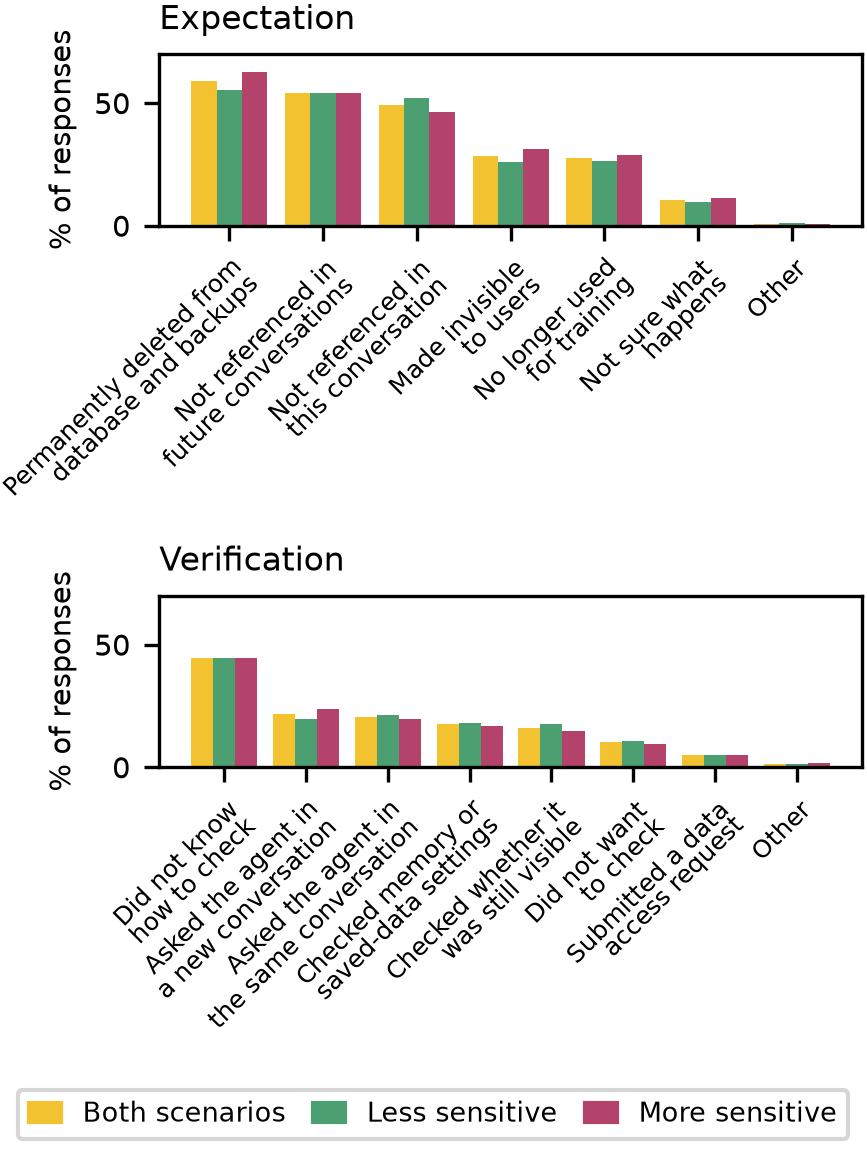
\includegraphics[width=\columnwidth,height=0.45\textheight,keepaspectratio]{figures/fig_expectation.png}
%     \caption{Expected deletion outcomes and reported verification strategies in LS, MS, and Pooled. The analysis includes 354 responses from 177 participants, with multiple selections allowed. Percentages are based on 177 participants within each scenario and 354 responses for Pooled results.}
%     \label{fig:expectation}
% \end{figure}


% \begin{figure*}[t]
%     \centering
%     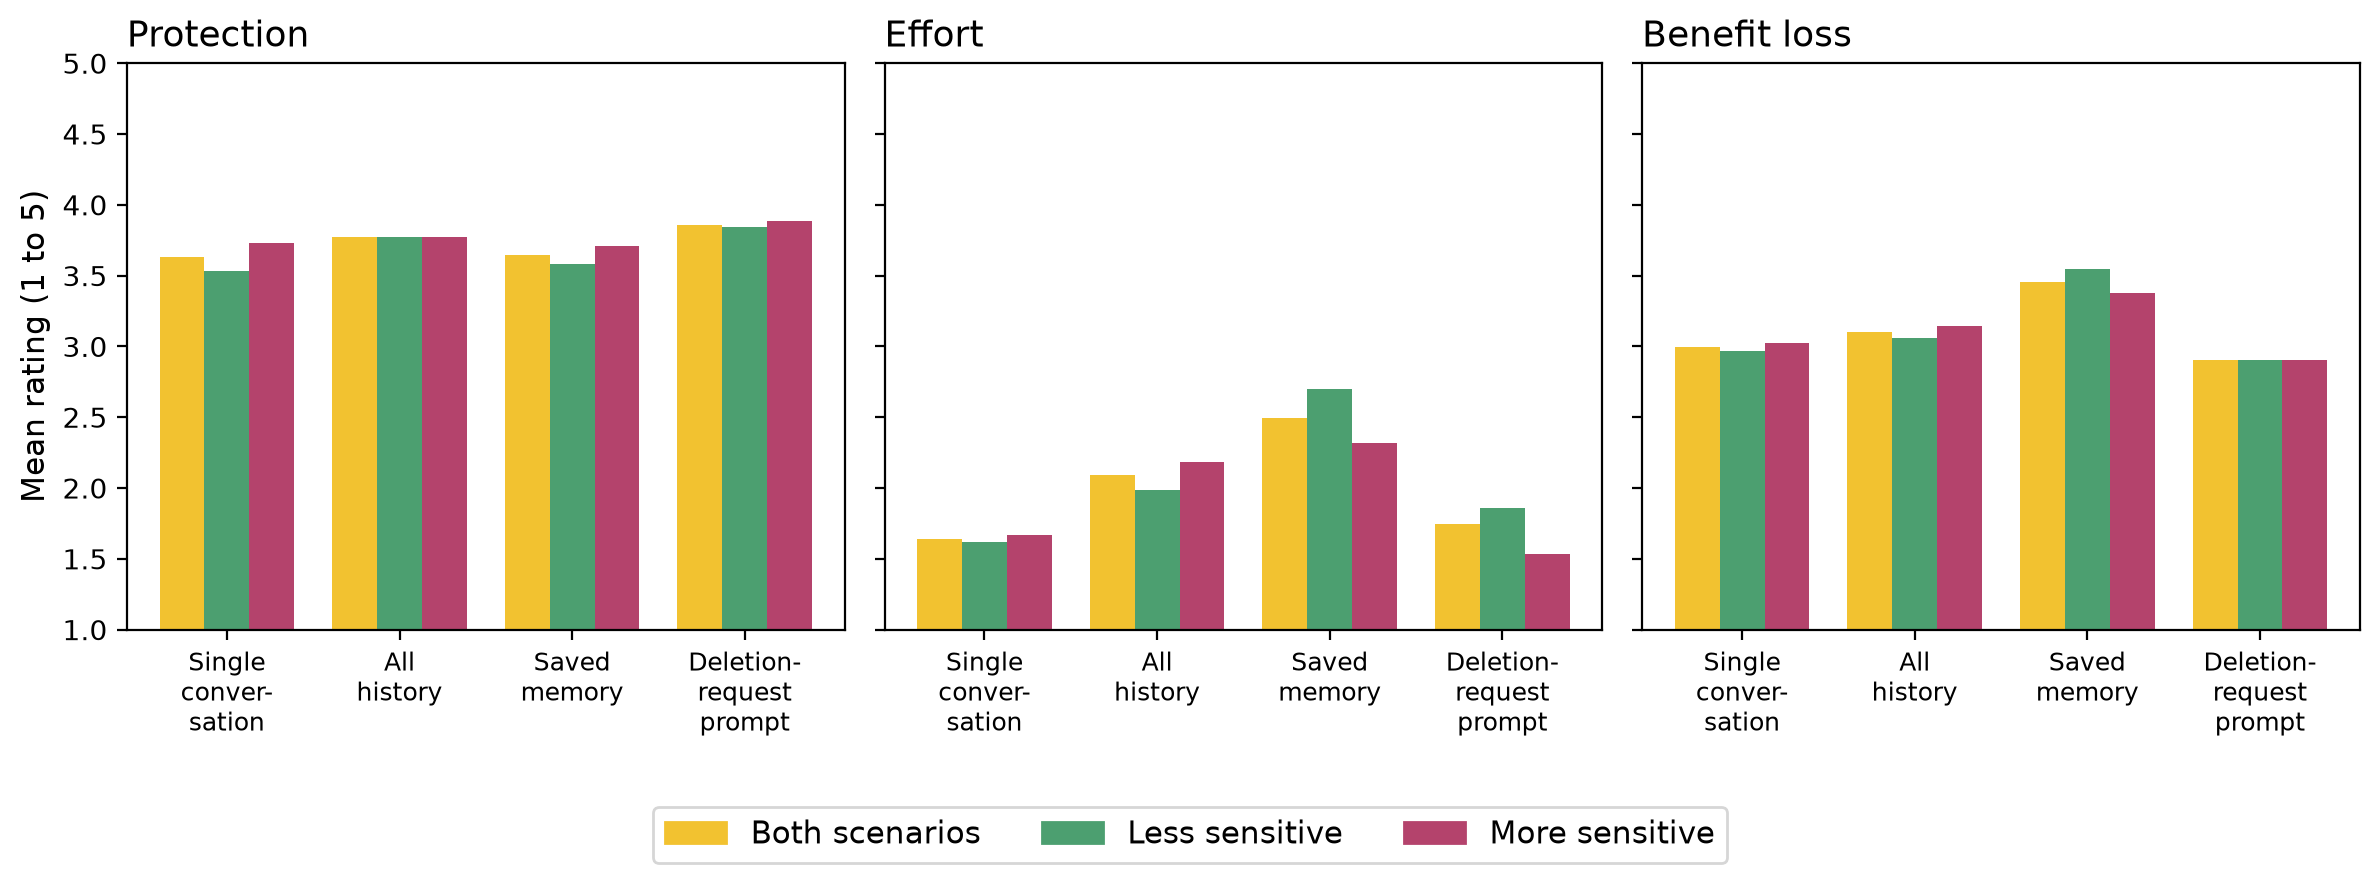
\includegraphics[width=0.94\textwidth]{figures/fig_scales.png}
%     \caption{Mean ratings of perceived privacy protection, effort, and potential loss of personalized benefits for the four most frequently selected deletion methods, shown separately for LS and MS and combined (Pooled). The analysis includes 317 responses from 105, 50, 30, and 29 participants, respectively. Ratings use five-point agreement scales.}
%     \label{fig:scales}
% \end{figure*}

% Many participants were uncertain how to verify deletion outcomes.
% %
% Across Pooled responses, 44.6\% indicated that they did not know how to verify deletion.
% %
% Reported verification strategies included asking the agent in the same or a new conversation (21\%--22\% of responses) and checking saved memories, settings, or the user interface (16\%--18\%).
% %
% Notably, among responses selecting a deletion-request prompt, 53.8\% (of 39 responses) indicated verification by asking the agent in the same conversation.
% %
% This suggests that users relying on conversational deletion requests may also rely on the agent's own responses as evidence that deletion succeeded.

% Participants also reported limitations in deletion feedback and experiences of information resurfacing.
% %
% Among the 177 participants, 42 (23.7\%) reported that an agent had referenced information they believed was deleted.
% %
% After previous deletion attempts, 41.2\% reported receiving a clear confirmation message, while 29.4\%--34.5\% reported vague acknowledgements or no feedback (multiple selections allowed).
% %
% Furthermore, 73 participants (41.2\%) wanted a breakdown specifying what information had been deleted and what might still be retained.
% %
% These findings highlight a gap between users' expectations of deletion and their ability to establish its outcome, motivating our subsequent post-deletion analysis (Section~\ref{sec:tech_analysis}).

% %
% \begin{takeawaybox}
% \textbf{Finding 2:} Participants commonly expected deletion methods to permanently remove their data, despite differences in the data locations these methods target. Perceived effort differed across methods, but expected deletion outcomes and perceived protection showed no significant differences. Many participants did not know how to verify deletion, and those selecting deletion-request prompts often relied on the agent itself for verification.
% \end{takeawaybox}



\section{Analyzing Post-Deletion Agent Behavior}
\label{sec:tech_analysis}
%
To investigate how commercial LLM agents respond to data deletion requests and whether previously disclosed information remains retrievable afterward (RQ3), we developed a new Data Injection-Deletion-Recall (DIDR) analysis pipeline.
%
We also compare observed agent behavior with users' deletion expectations (RQ4).
%
This section describes our methodology and presents the findings for RQ3 and RQ4.

\subsection{Post-Deletion Analysis Methodology}
%
Our methodology consists of three components: (1) the DIDR pipeline, which conducts controlled experiments across LLM agents and deletion methods using traceable synthetic facts; (2) outcome measures and analysis procedures for evaluating post-deletion agent behavior; and (3) comparisons between observed agent behavior and users' deletion expectations and verification strategies.
%
We describe each component in detail below.

\subsubsection{DIDR Analysis Pipeline}
%
\label{sec:didr}
%
As illustrated in Figure~\ref{fig:didr}, the DIDR pipeline comprises three stages: \textit{data injection}, which introduces a synthetic fact into an LLM agent; \textit{data deletion}, which applies a deletion method; and \textit{data recall}, which examines whether the injected fact remains retrievable afterward.
%
Each test case combines a synthetic fact, an injection method, a deletion method, and an LLM agent.
%
By injecting synthetic facts with unique values, we can attribute subsequent recall of those values to information introduced during our experiments.
%
The pipeline supports two complementary experimental approaches.
%
\textit{UI-action experiments} examine the information-entry and deletion controls available through each agent's interface, whereas \textit{prompt-based experiments} evaluate deletion requests authored by participants in our user study (Section~\ref{sec:user_study}).
%
In both approaches, deletion occurs at least 48 hours after injection, and recall testing occurs at least 30 days after deletion.
%
We chose this interval because several LLM agents (e.g., XX~\cite{}, XX~\cite{}, and XX~\cite{}) document that deleted data may remain in their systems for up to 30 days, and we applied the same interval across all agents for consistency.
%
We use Playwright-based automation~\cite{} for supported interactions and conduct the remaining operations manually.

\begin{figure*}[t]
    \centering
    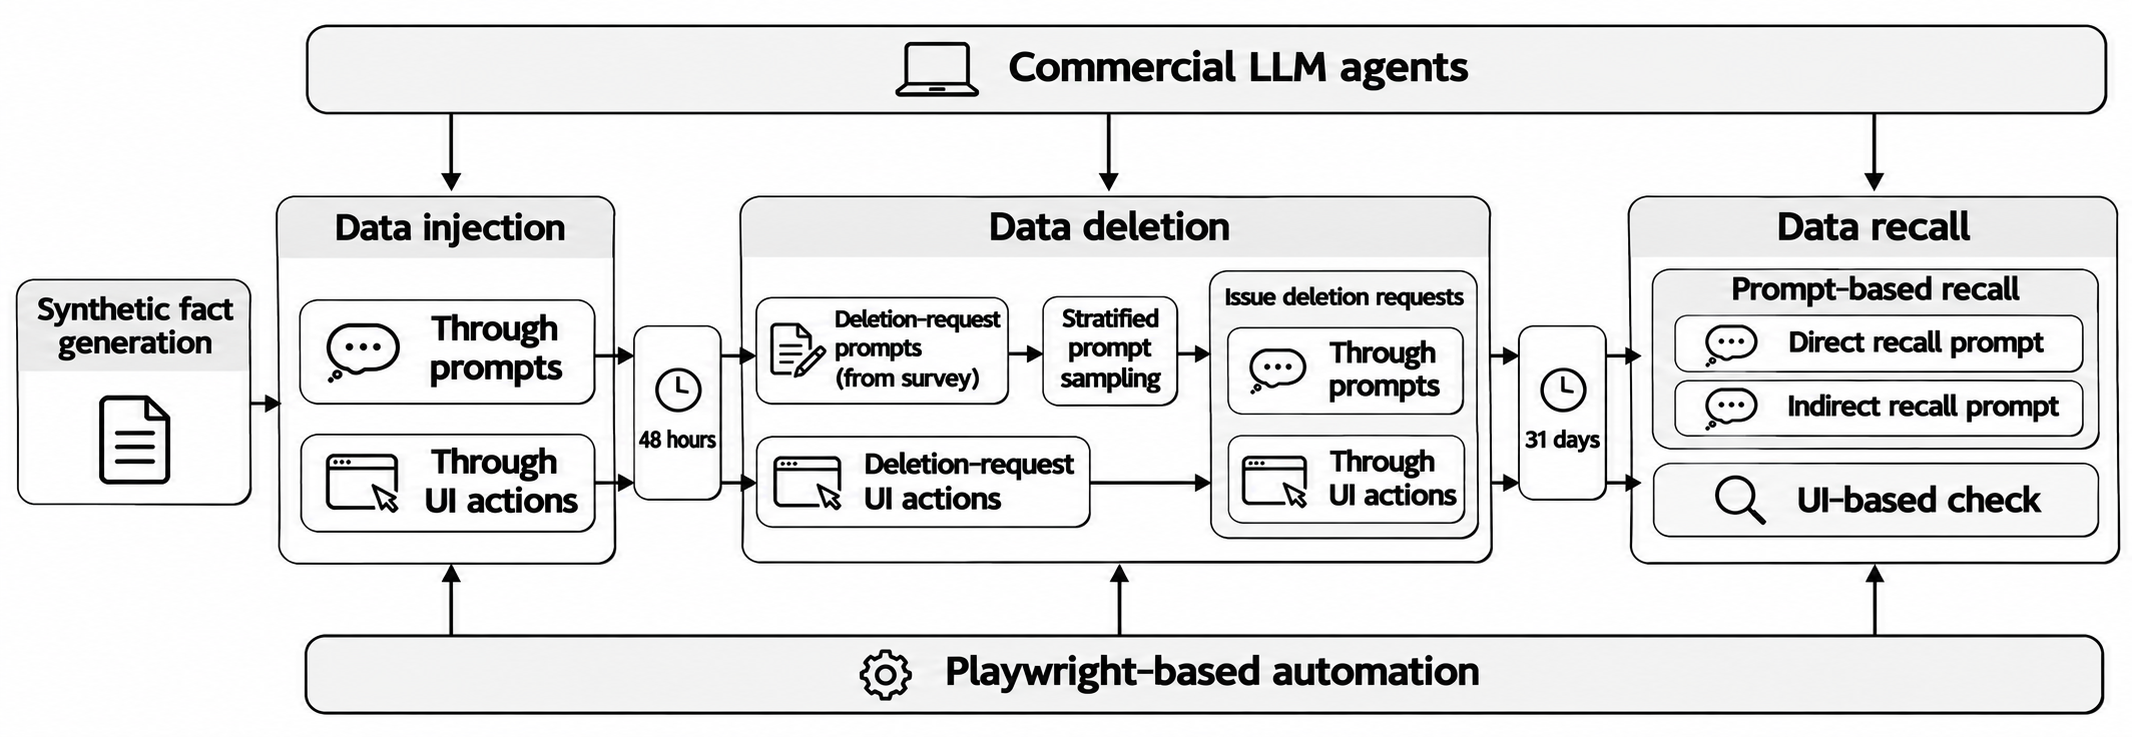
\includegraphics[width=\textwidth]{figures/DIDR.png}
    \caption{Overview of the DIDR analysis pipeline. Synthetic facts are injected into commercial LLM agents through prompts or UI actions, followed by deletion at least 48 hours later and recall testing at least 30 days after deletion. Deletion is performed using available agent controls or participant-authored deletion-request prompts, while recall is assessed through direct and indirect prompts and UI-based checks. Playwright automates supported interactions, with other operations performed manually.}
    \label{fig:didr}
\end{figure*}

\para{Synthetic fact generation}
%
To trace subsequent recall to a specific injected fact, we generated synthetic facts unlikely to have been previously encountered by LLM agents.
%
Each fact is represented as an $\langle$ \texttt{entity}, \texttt{attribute}, \texttt{value} $\rangle$ tuple, where the \texttt{entity} represents an everyday object or project, the \texttt{attribute} identifies a property, and the \texttt{value} is a unique synthetic code name comprising two to four words.
%
For example, one fact is $\langle$\textit{a scarf I'm knitting}, \textit{name}, ``\textit{Magnifier King Broom}''$\rangle$.
%
Following the canary-based approach of Carlini et al.~\cite{carlini2019secret}, each value is unique to one test case, allowing us to trace subsequent retrieval of the value to its corresponding injection.
%
We manually curated entities representing everyday objects and projects.
%
Values were generated using the EFF long word list~\cite{}, retaining words with a noun sense in WordNet~\cite{} while excluding terms associated with weapons, drugs, sexual content, and other potentially sensitive categories.
%
This filtering reduced the possibility that platform safety restrictions would interfere with recall observations.
%
Each fact was embedded in a casual conversational sentence, with wording varied across test cases to resemble ordinary user interactions.

\para{Data injection}
%
We injected synthetic facts through the \textit{information-entry} mechanisms supported by each LLM agent.
%
For UI-action experiments, we systematically examined each agent's web interface to identify available mechanisms, following an approach similar to prior walkthroughs of LLM privacy controls~\cite{li2026privacy}.
%
These mechanisms included \textit{casually disclosing information during a conversation}, \textit{explicitly requesting the agent to remember information}, and \textit{entering information through dedicated interfaces}, such as saved-memory pages~\cite{}, custom instructions~\cite{}, or saved-information pages~\cite{}.
%
We tested only the mechanisms available for each agent.
%
For prompt-based experiments, we held the injection method constant by introducing each fact as a casual statement in a conversation, allowing us to examine different deletion requests without varying how the information was initially disclosed.
%
In both approaches, we waited at least 48 hours before initiating deletion to allow time for the agent to process and potentially retain the injected information.

\para{Data deletion}
%
We evaluated deletion through two complementary approaches.
%
For UI-action experiments, we applied the deletion methods identified in our interface walkthrough (Table~\ref{tab:methods}), including UI-based controls targeting conversations, saved memories, and account-level data management.
%
This approach also included 13 test cases in which deletion was requested through a conversational prompt.
%
For each agent, we further tested its most extensive available deletion procedure by combining all applicable controls.
%
We excluded two methods included in the survey: \textit{deleting the account}, which would prevent subsequent observation of the same account, and \textit{filing a request with the company}, which is handled outside the agent.
%
Across the six agents, we designed 73 UI-action test cases and executed 67, as the remaining six required paid Perplexity features.
%
To prevent interference between test cases, we used dedicated accounts for deletion procedures that could affect other stored information.
%
Where multiple deletion procedures shared an account, we executed them from narrower to broader scopes (e.g., deleting a single conversation before clearing all conversation history) to avoid prematurely removing facts associated with other test cases.

For prompt-based experiments, we used deletion requests authored by survey participants to reflect how users express deletion intentions in natural language (i.e., participant-authored deletion-request prompts in Section~\ref{subsubsec:questions}).
%
In total, 209 participants provided 415 requests, including participants without prior deletion experience, as the prompt-writing task was hypothetical.
%
After removing duplicate and repeated requests, 375 distinct requests remained, and identifying information was redacted from seven requests.
%
Testing all 375 requests across six agents would have required 2,250 test cases under free-tier usage constraints.
%
Therefore, we grouped the requests into seven keyword-based categories according to references to deletion targets, such as memories, conversations, accounts, or databases, and selected 138 requests through stratified random sampling.
%
We selected at least 15 requests per category and included all requests from the two smallest categories to ensure coverage of less frequent formulations.


To characterize the selected requests, two researchers independently coded the 138 requests along seven dimensions: \textit{deletion location}, \textit{justification}, \textit{data named}, \textit{mood}, \textit{tone}, \textit{verb}, and \textit{accompanying request}.
%
They initially coded a subset of 50 requests independently without a shared codebook, reconciled their identified dimensions into a common codebook, and refined it through additional independent coding rounds.
%
They then independently coded all 138 requests and resolved disagreements through discussion.
%
Inter-rater agreement was high, with a pooled Gwet's AC1~\cite{gwet2008ac1} of 0.954 across the seven dimensions and at least 0.89 for each dimension (Table~\ref{tab:coding}).
%
The reconciled codes were subsequently used to examine associations between deletion-request wording and recall outcomes.


Five sampled requests asked agents to delete all user data and were excluded because they could interfere with other test cases.
%
We submitted the remaining 133 requests to all six agents, yielding 798 prompt-based test cases.
%
Together with the 67 executable UI-action test cases, our main evaluation comprised 865 test cases.
%
We separately designed 12 supplemental test cases involving uploaded files, examining conversation deletion and each agent's most extensive deletion procedure.
%
Eleven were executable, while the remaining case required a paid Perplexity feature.
%
These supplemental cases were analyzed separately because uploaded content may be accessible through the conversation context, saved memories, or both.

\begin{table}[t]
\centering
\caption{Inter-rater agreement for coding 138 participant-authored deletion requests. AC1 denotes Gwet's agreement coefficient.}
\label{tab:coding}
\small
\begin{tabular}{@{}lrrr@{}}
\toprule
Dimension & Agreed & \% & AC1 \\
\midrule
Deletion location & 125/138 & 90.6 & 0.890 \\
Justification & 131/138 & 94.9 & 0.943 \\
Data named & 133/138 & 96.4 & 0.956 \\
Mood & 133/138 & 96.4 & 0.959 \\
Tone & 137/138 & 99.3 & 0.990 \\
Verb & 131/138 & 94.9 & 0.947 \\
Accompanying request & 133/138 & 96.4 & 0.962 \\
\midrule
All dimensions (966 ratings) & 923/966 & 95.5 & 0.954 \\
\bottomrule
\end{tabular}
\end{table}

\para{Data recall}
%
We conducted recall testing at least 30 days after deletion.
%
This interval reflects documented periods during which deleted information may remain in the systems of ChatGPT, Claude, and Perplexity, and was applied consistently across all six agents for comparability.
%
We assessed post-deletion recall through three checks: \textit{direct recall prompts}, \textit{indirect recall prompts}, and \textit{UI-based checks}.
%
Direct prompts explicitly asked about the injected entity and its attribute, whereas indirect prompts requested an ordinary task involving the entity without mentioning the attribute or its value.
%
\xw{Provide an example here.}
%
These complementary checks allowed us to examine both explicitly requested retrieval and information resurfacing without a direct request for the injected fact.
%
Each prompt type was issued twice using different wording to reduce dependence on a single formulation.
%
We searched the resulting responses for injected values and manually reviewed the outputs.

UI-based checks examined whether the injected information remained visible in the agent's saved-memory or saved-information interface.
%
These checks were performed where such interfaces were available and omitted for DeepSeek, Perplexity, and Copilot accounts without accessible memory pages.
%
To minimize interference between recall checks, we first inspected the interface, followed by indirect and direct recall prompts in a new conversation.
%
When deletion was requested in the original conversation, we also issued the first direct recall prompt in that conversation and reported the result separately, since the original disclosure could remain available in its conversational context.

\subsubsection{Outcome Measures and Analysis}
\label{sec:didr_analysis}
%
We evaluated post-deletion agent behavior using multiple measures, including agents' responses to deletion requests, the retrievability of injected information, observable interface changes, and consistency with published documentation.
%
We also examined whether the wording of participant-authored deletion requests was associated with recall outcomes.
%
Importantly, these measures characterize externally observable behavior rather than establishing complete erasure of information from an agent's underlying systems.

\para{Deletion-request responses}
%
We analyzed agents' responses to deletion requests submitted through chat to characterize their stated handling of the requests.
%
Through an initial review of the responses, we identified recurring patterns and developed six categories: \textit{complied}, \textit{partial}, \textit{deflected}, \textit{refused}, \textit{silently ignored}, and \textit{other}.
%
A response was classified as \textit{complied} if the agent confirmed completion without stating limitations or redirecting the user.
%
It was classified as \textit{partial} if the agent confirmed an action but stated limitations, redirected the remaining steps, or merely promised not to use the information.
%
A response was \textit{deflected} if the agent redirected the user without confirming any deletion action, and \textit{refused} if it stated that deletion could not or would not be performed without providing a redirect.
%
Responses that engaged with the conversation without acknowledging the deletion request were classified as \textit{silently ignored}.
%
Other responses, including clarification questions, permission prompts, and usage-limit messages, were classified as \textit{other}.
%
Two researchers independently coded the responses based only on the agents' statements, without inferring whether deletion actually occurred.
%
They agreed on 767 of 788 responses (Gwet's AC1 = 0.969), resolving disagreements through discussion.
%
UI-based deletion actions without conversational responses were excluded from this analysis.

\para{Recall outcome classification}
%
We classified each test case into one of three outcomes: \textit{recall success}, \textit{recall failed}, or \textit{can't tell}.
%
A test case was classified as \textit{recall success} if any applicable recall check retrieved the injected value.
%
It was classified as \textit{recall failed} only if no recall check retrieved the value and there was evidence that the fact had initially been saved in the tested location.
%
Otherwise, the outcome was classified as \textit{can't tell}.
%
This distinction prevents the inability to retrieve a fact from being interpreted as evidence of successful deletion when its initial storage cannot be verified.

%
We assessed initial storage using agent responses and screenshots recorded during injection.
%
A fact was considered saved only when the interface displayed an explicit memory notification, such as ``\textit{Memory updated},'' or the agent explicitly confirmed saving the information.
%
Generic acknowledgments, such as ``\textit{Got it},'' were insufficient, and ambiguous responses were manually reviewed.
%
We also identified responses in which agents withheld information because of earlier deletion or non-use requests, using phrase matching followed by manual verification.
%
Such responses were recorded separately and did not change the recall classification.

%
For UI-action experiments, we further examined whether the relevant interface reflected the requested deletion, such as a conversation disappearing from history or a saved fact disappearing from memory.
%
We assessed these changes through post-deletion screenshots and directly inspected accounts when the screenshots were inconclusive.
%
Comparable interface changes were not observable for deletion requests submitted through chat.
%
These observations provide evidence about externally visible deletion behavior but do not independently establish complete removal from an agent's underlying storage.

\para{Documentation consistency}
%
We examined whether observed post-deletion behavior was consistent with each agent's published help and privacy documentation.
%
For each test case, we classified the documented commitment associated with its deletion method and injection location into five categories: \textit{deletes}, \textit{does not delete}, \textit{no commitment}, \textit{unrelated}, and \textit{not testable}.
%
We issued consistency verdicts only when documentation explicitly stated that the method would remove the relevant information (\textit{deletes}) or would not remove it (\textit{does not delete}).
%
For a \textit{deletes} commitment, recall success or an unchanged interface contradicted the documented behavior, whereas recall failed with a changed or unobservable interface was considered consistent.
%
Recall from the original conversation alone was also considered consistent when the documentation stated that previous conversations would remain accessible.
%
For a \textit{does not delete} commitment, recall success was considered consistent with the documentation.
%
Cases classified as \textit{can't tell} remained unresolved, and the remaining commitment categories received no consistency verdict.


\para{Deletion-request wording}
\label{par:request_wording}
%
Using the seven coding dimensions described above, we examined whether participant-authored deletion-request wording was associated with recall outcomes within each agent.
%
Because some coding categories contained relatively few requests, we reported descriptive recall-success counts without statistical tests and restricted comparisons to categories containing at least six deletion requests.
%
Agents whose test cases were all classified as \textit{can't tell} were excluded from these comparisons.

\begin{table}[t]
\centering
\caption{Inter-rater agreement for coding 138 participant-authored deletion requests. AC1 denotes Gwet's agreement coefficient.}
\label{tab:coding}
\small
\begin{tabular}{@{}lrrr@{}}
\toprule
Dimension & Agreed & \% & AC1 \\
\midrule
Deletion location & 125/138 & 90.6 & 0.890 \\
Justification & 131/138 & 94.9 & 0.943 \\
Data named & 133/138 & 96.4 & 0.956 \\
Mood & 133/138 & 96.4 & 0.959 \\
Tone & 137/138 & 99.3 & 0.990 \\
Verb & 131/138 & 94.9 & 0.947 \\
Accompanying request & 133/138 & 96.4 & 0.962 \\
\midrule
All dimensions (966 ratings) & 923/966 & 95.5 & 0.954 \\
\bottomrule
\end{tabular}
\end{table}


\subsubsection{Comparing User Expectations with Agent Behavior}
\label{sec:expectation_behavior}
%
To examine the alignment between users' deletion expectations and observed agent behavior (RQ4), we compared the survey findings with DIDR test cases involving corresponding deletion methods.
%
Because survey percentages represent participants' responses whereas experimental percentages represent test cases, we compared patterns rather than treating the percentages as directly equivalent.
%
We conducted two comparisons.
%
First, we compared users' expectations that deleted information would not resurface in future conversations with observed recall outcomes.
%
Recall success contradicted this expectation, whereas recall failed was consistent with it.
%
We focused on future-conversation recall because it was observable across the DIDR test cases, whereas other expectations, such as permanent removal from databases and backups or exclusion from model training, could not be directly assessed through external testing.
%
Second, we examined whether the signals participants reported using to verify deletion corresponded to the observed outcomes.
%
These signals included agents' responses to deletion requests, their responses to subsequent queries in the original conversation, and observable changes to the user interface.
%
This comparison allowed us to assess whether commonly used verification strategies provided reliable indications of post-deletion agent behavior.



\subsection{Post-Deletion Analysis Findings}
\label{sec:tech_results}
%
We present the results of our DIDR analysis, focusing on post-deletion agent behavior (RQ3) and its alignment with users' deletion expectations and verification strategies (RQ4).
%
We distinguish among \textit{recall success}, \textit{recall failed}, and \textit{can't tell}, as defined in Section~\ref{sec:didr_analysis}.


\subsubsection{Post-Deletion Agent Behavior (RQ3)}

Post-deletion recall outcomes were often uncertain, and previously disclosed information remained retrievable in a substantial number of test cases.
%
Of the 865 test cases, 394 (45.5\%) had determinable recall outcomes, including 162 (41.1\% of determinable cases) classified as \textit{recall success}.
%
The remaining 471 test cases (54.5\%) were classified as \textit{can't tell} because we could not establish that the injected facts had initially been saved in the tested locations.
%
Thus, recall success was observed in 18.7\% of all test cases, while more than half could not support a definitive recall outcome.

%
No deletion method consistently prevented recall across all determinable test cases.
%
Among the four methods evaluated through UI actions, recall success occurred in 29\%--50\% of test cases, although the small sample sizes (7--13 cases per method) do not support reliable rankings.
%
For deletion-request prompts, the most extensively tested method, 144 of 811 test cases resulted in recall success, while 454 were classified as \textit{can't tell}.
%
We separately evaluated 12 supplemental uploaded-file test cases, of which 11 were executable because one Perplexity procedure required a paid plan.
%
In all 11 executable cases, the injected facts were not retrieved in subsequent conversations, and the test cases were classified as \textit{recall failed}.

\begin{takeawaybox}
\textbf{Finding 3:} Previously disclosed information remained retrievable after deletion in a substantial number of test cases. However, 54.5\% of outcomes were inconclusive because initial storage could not be verified, highlighting the difficulty of determining deletion outcomes through external testing.
\end{takeawaybox}

\begin{table}[!t]
\centering
\caption{Post-deletion recall outcomes across the six LLM agents (865 test cases).}
\label{tab:outcomes-agent}
\footnotesize
\begin{tabular}{@{}lrrrr@{}}
\toprule
Agent & Recall success & Recall failed & Can't tell & Test cases \\
\midrule
ChatGPT & 118 & 28 & 5 & 151 \\
Claude & 3 & 141 & 4 & 148 \\
Copilot & 5 & 59 & 81 & 145 \\
DeepSeek & 0 & 0 & 137 & 137 \\
Gemini & 5 & 2 & 138 & 145 \\
Perplexity & 31 & 2 & 106 & 139 \\
\midrule
Total & 162 & 232 & 471 & 865 \\
\bottomrule
\end{tabular}
\end{table}

\para{Differences across LLM agents}
%
Post-deletion recall outcomes differed substantially across LLM agents (Table~\ref{tab:outcomes-agent}).
%
ChatGPT accounted for 118 of the 162 recall-success cases, whereas Claude exhibited predominantly recall-failed outcomes (141 of 148 cases).
%
Copilot also had more recall-failed than recall-success outcomes among its determinable cases.
%
In contrast, the majority of test cases for Gemini, Perplexity, and DeepSeek were classified as \textit{can't tell}, limiting conclusions about their deletion effectiveness.
%
Differences were also evident for deletion requests submitted through chat.
%
Among cases with determinable outcomes, Claude and Copilot generally did not retrieve the injected facts, whereas ChatGPT frequently retrieved them.
%
Perplexity exhibited both recall-success and uncertain outcomes, while all prompt-based test cases for Gemini and DeepSeek were classified as \textit{can't tell}.
%
These patterns indicate substantial variation across agents in observable post-deletion recall.

%
Some differences were consistent with the locations in which agents retain information and the scope of their deletion controls.
%
For example, Claude's documentation states that deleting a conversation does not remove memory entries created from that conversation.
%
Consistent with this distinction, deleting a conversation resulted in recall success in all three corresponding UI-action test cases, whereas deleting a saved memory resulted in recall failed in all three.
%
On ChatGPT, the saved-memory interface no longer displayed the injected fact in 112 of the 118 recall-success cases, indicating that the observed recall could not be attributed solely to a visible saved-memory entry.
%
DeepSeek did not provide an accessible memory interface or sufficient evidence of initial storage, leaving all its test cases classified as \textit{can't tell}.

\para{Deletion-request wording}
%
We examined whether participant-authored deletion-request wording was associated with recall outcomes.
%
Among the 350 prompt-based test cases with determinable outcomes, we compared recall outcomes across the seven manually coded wording dimensions, including deletion location, justification, mood, and tone.
%
On Claude and Copilot, recall success did not occur within any coding category in these comparisons, while on ChatGPT it occurred in at least half of the test cases for every category containing six or more requests.
%
Perplexity exhibited greater variation across categories, although categories showing differences generally contained few requests.
%
Gemini and DeepSeek were excluded because all their prompt-based cases were classified as \textit{can't tell}.
%
These descriptive results suggest that differences across agents were more pronounced than differences associated with request wording, although they do not establish that wording has no effect.

\begin{takeawaybox}
\textbf{Finding 4:} Post-deletion recall varied substantially across LLM agents, with differences consistent in some cases with their data-storage mechanisms and deletion controls. In contrast, deletion-request wording showed no consistent pattern that explained these cross-agent differences.
\end{takeawaybox}


\para{Documentation consistency}
%
Observed post-deletion behavior was largely consistent with agents' published documentation, even when previously disclosed information remained retrievable.
%
Among deletion requests submitted through chat, 319 test cases received a documentation-consistency verdict, of which 318 were consistent and one contradicted the documented behavior.
%
Notably, 107 of the consistent cases were classified as \textit{recall success}, all involving ChatGPT, whose documentation states that deleting a saved memory does not remove mentions of that information from previous conversations.
%
For Gemini, Perplexity, and DeepSeek, the relevant documentation did not provide an applicable commitment for these requests.
%
Among UI-action test cases, 22 of the 23 cases with a verdict were consistent with documentation, including six classified as \textit{recall success}.

\begin{takeawaybox}
\textbf{Finding 5:} Observed behavior was usually consistent with applicable deletion documentation, even when information remained retrievable. This suggests that, by design, some agents' deletion mechanisms have limited scopes that do not necessarily prevent previously disclosed information from resurfacing in future conversations.
\end{takeawaybox}


\para{Agent responses to deletion requests}
%
Agents' responses to deletion requests did not reliably indicate subsequent recall outcomes.
%
Among the 798 deletion requests evaluated in the prompt-based experiments, 566 (70.9\%) received responses classified as \textit{complied} or \textit{partial}.
%
Of these, 112 (19.8\%) resulted in \textit{recall success}, including 11 cases following \textit{complied} responses and 101 following \textit{partial} responses (Table~\ref{tab:replies-outcome}).
%
Among cases with determinable outcomes, \textit{complied} or \textit{partial} responses were generally associated with \textit{recall failed} on Claude and Copilot but frequently with \textit{recall success} on ChatGPT and Perplexity.
%
These findings indicate that agents' responses acknowledging deletion, even when indicating full compliance, do not necessarily establish that previously disclosed information is no longer retrievable.


\begin{table}[!t]
\centering
\caption{Post-deletion recall outcomes by agents' responses to participant-authored deletion requests (798 test cases).}
\label{tab:replies-outcome}
\footnotesize
\begin{tabular}{@{}lrrrr@{}}
\toprule
Response & Recall success & Recall failed & Can't tell & Test cases \\
\midrule
Complied & 11 & 142 & 146 & 299 \\
Partial & 101 & 39 & 127 & 267 \\
Deflected & 13 & 11 & 144 & 168 \\
Refused & 1 & 0 & 7 & 8 \\
Silently ignored & 3 & 1 & 3 & 7 \\
Other & 10 & 18 & 21 & 49 \\
\midrule
Total & 139 & 211 & 448 & 798 \\
\bottomrule
\end{tabular}
\end{table}

%
Some agents explicitly withheld information because of an earlier deletion or non-use request.
%
For example, an agent responded, ``I can't provide that name because you previously asked me to delete the information about your letterpress kit.''
%
Among test cases without recall success, such responses occurred in 52\%--95\% of cases on ChatGPT and Perplexity, but not on the other four agents.
%
For Perplexity in particular, these responses accounted for many cases classified as \textit{can't tell}, illustrating that an agent's refusal to disclose information does not establish that the underlying fact was erased.

%
We also observed agent-specific responses unrelated to direct deletion confirmation.
%
For example, Gemini displayed an application-permission card in 6.0\% of its prompt-based deletion requests, particularly when requests concerned projects or plans.
%
These requests may have been interpreted as instructions to delete information in a connected Google application.
%
We declined all such permission requests, and the corresponding test cases were classified as \textit{can't tell}.

\begin{takeawaybox}
\textbf{Finding 6:} Agent responses acknowledging deletion did not reliably indicate subsequent recall outcomes. Previously disclosed information remained retrievable in some cases even after agents indicated full compliance with deletion requests.
\end{takeawaybox}


\subsubsection{User Expectations vs. Agent Behavior (RQ4)}
\label{sec:expectation}

Users commonly expected deletion methods to prevent previously disclosed information from resurfacing in future conversations, but the DIDR experiments showed that this expectation was not consistently met.
%
For the four most frequently selected deletion methods, 42.5\%--63.4\% of Pooled survey responses expected the agent to no longer reference the deleted information in future conversations (Section~\ref{sec:qual_results}).
%
However, each of these methods produced recall-success outcomes in at least some test cases (Table~\ref{tab:expectation-outcome}).
%
For example, deleting a single conversation resulted in recall success in six of 13 test cases, while clearing all conversation history resulted in recall success in four of eight.

%
Deletion-request prompts exhibited similar discrepancies, although uncertainty was substantial.
%
Among the 811 test cases using this method, 144 resulted in recall success, 213 in recall failed, and 454 in \textit{can't tell}.
%
Thus, observable recall contradicted the expectation that deletion would prevent subsequent retrieval in some cases, while more than half of these outcomes could not be determined.
%
Because the survey reports shares of participant responses and the DIDR analysis reports shares of experimental test cases, these values describe different populations of observations and should not be interpreted as directly comparable rates.

\begin{table}[!t]
\centering
\caption{Survey expectations that information would not resurface in future conversations and observed DIDR recall outcomes, by deletion method. Expectations are percentages of Pooled survey responses; outcomes are numbers of experimental test cases.}
\label{tab:expectation-outcome}
\footnotesize
\setlength{\tabcolsep}{3pt}
\begin{tabularx}{\columnwidth}{@{}Xrrrrr@{}}
\toprule
Method & Expected & \makecell[r]{Recall\\success} & \makecell[r]{Recall\\failed} & \makecell[r]{Can't\\tell} & \makecell[r]{Test\\cases} \\
\midrule
Delete a single conversation & 54.3\% & 6 & 1 & 6 & 13 \\
Clear all conversation history & 42.5\% & 4 & 2 & 2 & 8 \\
Delete a specific saved memory & 63.4\% & 2 & 3 & 2 & 7 \\
Send a deletion-request prompt & 51.3\% & 144 & 213 & 454 & 811 \\
\bottomrule
\end{tabularx}
\end{table}

%
Participants also commonly expected permanent deletion from databases and backups (52.1\%--65.9\% across the four methods).
%
Although recall success provides evidence inconsistent with complete removal of the retrieved information, recall failed cannot confirm permanent deletion from underlying databases or backups.
%
Therefore, our comparison focuses primarily on the expectation that deleted information will not resurface in future conversations, which can be assessed through the DIDR recall checks.

%
Our documentation analysis provides further context for these discrepancies.
%
Some recall-success outcomes were consistent with agents' published deletion commitments, indicating that documented deletion scopes may be narrower than users' expectations.
%
Moreover, several agents did not provide applicable commitments for conversational deletion requests, making it difficult for users to determine what such requests actually accomplish.

\begin{takeawaybox}
\textbf{Finding 7:} Users expected deletion to prevent previously disclosed information from resurfacing in future conversations. However, all four evaluated deletion methods resulted in recall success in some test cases, contradicting this expectation.
\end{takeawaybox}


\para{Verification signals vs. observed recall}
%
Users' reported verification strategies did not reliably establish whether previously disclosed information would resurface in future conversations.
%
Participants reported relying on conversational feedback and follow-up queries, while others looked for observable changes in the interface.
%
However, our DIDR experiments revealed limitations in each of these signals.
%
As shown in RQ3, agents sometimes indicated compliance with deletion requests even when the injected information remained retrievable.
%
Similarly, 53.8\% of survey responses selecting deletion-request prompts reported verification by asking the agent again in the same conversation.
%
Yet responses to such queries disagreed with subsequent recall outcomes in 26\%--78\% of determinable cases, depending on the agent.
%
For example, ChatGPT sometimes withheld information in the original conversation that remained retrievable in a new conversation, whereas Claude sometimes returned information in the original conversation despite a recall-failed outcome in the new-conversation evaluation.
%
Observable interface changes were also insufficient.
%
Among UI-action test cases with both visible interface changes and determinable recall outcomes, 42\% resulted in \textit{recall success}, despite the disappearance of conversations or memory entries from the interface.
%
These limitations help explain the verification uncertainty reported in our user study, where 44.6\% of Pooled responses indicated that participants did not know how to verify deletion.

\begin{takeawaybox}
\textbf{Finding 8:} Users lacked reliable ways to verify deletion. Agent confirmations, follow-up queries, and interface changes could indicate that deletion had occurred even when previously disclosed information remained retrievable in future conversations.
\end{takeawaybox}
\section{Discussion}
\label{sec:discussion}

\begin{outlinenote}
\begin{enumerate}[leftmargin=*,nosep]
\item Opening, no heading, two sentences: the one major finding . Users expect deletion to mean gone and cannot check it, and what happened depended on the agent, not on the wording.
\item Subsection: What Explains the Differences Across Agents. Where each agent keeps the fact and which data deletion method reaches that place; what each agent's documentation says a method removes, set against what we observed; regulation (we looked for a difference and report what we found, or that none distinguishes the agents). Explanations are worded as consistent with the observations, because the audit is black-box.
\item Subsection: Why Users Cannot Tell. The check users reach for first misleads; the agent's reply and the interface do not show the outcome. This joins the survey (expectation, check) to the audit. [Heading wording open.]
\item Subsection: What Each Party Should Do, by audience. Platforms: state what each data deletion method removes, say what a deletion did and did not do, and give users a way to check. Regulators: deletion rights have to be testable (no claim of GDPR compliance or non-compliance). Users: which methods reached what we tested, marked provisional. Researchers: the audit method and data are available. A table follows (as in Khandelwal et al.), with three columns: what we found, what we recommend, who acts. Each row traces a recommendation to a result section.
\item Subsection: Limitations, short and last, no new heading level. The survey describes US Prolific users of the six agents; free-tier accounts and one time window; prompt-based recall is weak evidence that a fact is gone; the can't tell share (provisional until recall finishes); the audit reports what a user can observe, not what a platform stores. The free-text reasons participants gave (not coded) go here as a note without counts.
\item Left out: repeated numbers (Sections 4 and 5 hold them), future work (Conclusion), related work (its own section).
\end{enumerate}
\end{outlinenote}

\section{Related Work}
\label{sec:related}



% 1. Systems and the law
% 2. Audits of deployed services
% 3. Unlearning and verification
% 4. Memorization and agent memory
% 5. Users and deletion controls
% 6. Users of LLM agents


% \begin{outlinenote}
% Plan: a wide and deep review of papers, published venues only , each verified against the publisher or proceedings page before it is cited.
% \begin{enumerate}[leftmargin=*,nosep]
% \item Data deletion in computer systems: What deletion means formally, and how software systems, databases, storage, websites, and web applications implement data deletion, including where the right to be forgotten has been applied outside language models.
% \item Audits of deployed services, about 10 papers. Technical analyses of whether websites, mobile apps, and other platforms delete data when asked.
% \item Deletion in AI: Machine unlearning methods, attacks on unlearning, how unlearning is verified, memorization of training data, and whether unlearning can be made usable by users.
% \item Users:. How users perceive privacy and memory in AI systems, how usable and effective deletion and privacy controls are, and how users verify that their data was removed.
% \item Gaps. Prior work audits services, studies unlearning inside models, and studies how users use controls. No work tests what happens after a deletion request to deployed LLM agents, or compares the outcome with what users expect and how they try to verify it.
% \end{enumerate}
% \end{outlinenote}


\para{Data deletion effectiveness and usability}
%
Prior research has examined the effectiveness and usability of data deletion across systems (mostly in domains other than LLM agents).
%
For example, secure deletion research shows that removing a file or issuing a deletion command does not necessarily eliminate the underlying data~\cite{reardon2013sok}.
%
Similar challenges arise in databases, where physical removal may be delayed~\cite{sarkar2020lethe,shastri2020understanding}, and in backups that fail to support the right to be forgotten~\cite{politou2018backups}.
%
Studies of deployed services have also identified gaps between deletion controls and actual outcomes.
%
Habib et al.~\cite{habib2019empirical} identified limitations in how websites present and explain deletion and opt-out choices, while other studies found that online services and mobile applications may retain personal information after deletion requests or account deletion~\cite{rupp2022leave,santhanam2022scraping,yan2025sign}.
%
These findings highlight the need to evaluate deletion outcomes rather than assume that available controls ensure data removal.

Beyond deletion effectiveness, usable privacy research further shows that users struggle to locate and exercise deletion controls~\cite{ramokapane2017stupid,habib2020scavenger,bumiller2026zombies}, and that their expectations may differ from what services provide~\cite{rao2016expecting}.
%
Minaei et al.~\cite{minaei2022deletion} also identified limitations in deletion privacy through users' experiences and expectations.
%
These usability studies are loosely related to our work, as they may affect how users choose, understand, and verify data deletion.

\para{Unlearning in machine learning}
%
Machine unlearning aims to remove the influence of selected training data from learned models.
%
Prior work has developed formal definitions~\cite{garg2020formalizing}, methods that avoid complete retraining~\cite{cao2015towards,bourtoule2021machine}, and certified removal guarantees under specific assumptions~\cite{guo2020certified}, with surveys summarizing these advances~\cite{xu2023machine}.
%
However, verification remains challenging~\cite{thudi2022necessity,xue2026towards}.
%
Evaluations of language-model unlearning reveal persistent privacy risks, including information leakage after unlearning~\cite{shi2025muse,patil2024sensitive}.
%
In-context unlearning can also modify model behavior without removing information from model parameters~\cite{pawelczyk2024incontext}, illustrating why non-retrieval does not necessarily establish erasure.
%
Related research shows that language models can memorize and reproduce training data~\cite{carlini2019secret,carlini2021extracting,carlini2023quantifying,lukas2023analyzing}.
%
Controlled insertion and extraction of synthetic information provides a useful way to investigate memorization~\cite{carlini2019secret}.
%
Building on this principle, our study examines a different setting: whether user-provided information remains retrievable after deletion through the controls of deployed LLM agents, rather than unlearning from model parameters.

\para{Data deletion in LLM agents}
%
LLM agents introduce additional privacy challenges by retaining user interactions and derived information.
%
As shown in past research, generative agents can store past interactions and generate reflections~\cite{park2023generative}, while agent memory can expose private information to extraction attacks~\cite{wang2025unveiling}, raising questions about whether deletion controls cover retained and derived data.
%
Recent studies have examined privacy controls and user perceptions in conversational LLM platforms.
%
For example, Li et al.~\cite{li2026privacy} studied six platforms, identifying challenges in accessing, editing, deleting, and sharing conversational data, including ambiguity in natural-language privacy controls.
%
Other work examined users' privacy concerns, disclosure decisions, and expectations~\cite{zhang2024fair,malki2025hoovered,kwesi2026impact}, while studies of ChatGPT memory and retrieval-augmented memory highlighted tensions between personalization and privacy~\cite{chen2026relational,zhang2025understanding}.
%
Despite these advances, limited empirical evidence connects users' deletion expectations with the observed post-deletion behavior of commercial LLM agents.
%
Our study addresses this gap by combining a user survey with controlled post-deletion recall experiments to evaluate information retrievability after different deletion methods and compare observed outcomes with user expectations and platform documentation.
\section{Conclusion}
\label{sec:conclusion}

We studied what happens when a user asks an LLM agent to delete data, from two sides: what users do and expect, and what six agents do afterward. In the survey, more sensitive data raised participants' willingness to delete but not which data deletion method they chose, and about half named sending a deletion-request prompt as ideal although few chose it. Most expected every data deletion method to delete permanently, and many did not know how to verify that it worked. In the post-deletion analysis, deletion did not reliably keep a fact out of later conversations, and what happened depended more on the agent than on the data deletion method or how the request was worded. Where we could judge, the fact stayed out of later conversations on Claude and Copilot and was often recall success on ChatGPT and Perplexity, and more than half of the deletions we tested were can't tell.

Users and agents differed where an agent kept a fact after a deletion that participants expected to keep out of later conversations. The signals participants relied on to verify a deletion, the agent's reply, asking again in the same conversation, and the interface, did not show which case a user was in. So deletion controls need to state what they act on and give users a way to verify the outcome. Future work can inspect what a platform stores, which needs access that platforms do not give, and can repeat the test on other agents, on paid plans, and with other types of data.


\bibliographystyle{IEEEtran}
\bibliography{refs}

\appendices

\begin{table}[t]
\centering
\caption{Participant demographics ($N=177$).}
\label{tab:demographics}
\small
\begin{tabular}{@{}lrr@{}}
\toprule
 & Count & \% \\
\midrule
\multicolumn{3}{@{}l}{\textit{Age}} \\
18--24 years & 29 & 16.4 \\
25--34 years & 56 & 31.6 \\
35--44 years & 45 & 25.4 \\
45--54 years & 27 & 15.3 \\
55--64 years & 17 & 9.6 \\
65+ years & 3 & 1.7 \\
\midrule
\multicolumn{3}{@{}l}{\textit{Gender}} \\
Man & 104 & 58.8 \\
Woman & 72 & 40.7 \\
Prefer not to say & 1 & 0.6 \\
\midrule
\multicolumn{3}{@{}l}{\textit{Education}} \\
Bachelor's degree & 75 & 42.4 \\
Graduate or professional degree & 35 & 19.8 \\
Some college, but no degree & 30 & 16.9 \\
Associate's or technical degree & 19 & 10.7 \\
High school diploma or GED & 15 & 8.5 \\
Some high school or less & 3 & 1.7 \\
\bottomrule
\end{tabular}
\end{table}

\section{Survey Questions}
\label{app:questions}

\end{document}